\documentclass{book}

\usepackage[utf8]{inputenc}
%\usepackage[english]{babel}
\usepackage[T2A]{fontenc}
\usepackage{tabularx}
\usepackage{amsmath,mathrsfs,amssymb}
\usepackage{bbding}
\usepackage{alltt}
\usepackage{epigraph}
\usepackage{verbatim}
\usepackage{soul}
\usepackage{latexsym}
\usepackage{array}
\usepackage{comment}
\usepackage{makeidx}
\usepackage{listings}
\usepackage{indentfirst}
\usepackage{verbatim}
\usepackage{color}
\usepackage{url}
\usepackage{xspace}
\usepackage{hyperref}
\usepackage{stmaryrd}
\usepackage{tikz}
\usetikzlibrary{arrows,decorations.pathreplacing,backgrounds,fit,positioning,shapes,chains,calligraphy,arrows.meta,shapes.arrows,overlay-beamer-styles}
\usepackage{euscript}
\usepackage{mathtools}
\usepackage{graphicx}
\usepackage{euscript}
\usepackage{mathtools}
\usepackage{transparent}
\usepackage{bold-extra}
\usepackage{subcaption}
\usepackage{placeins}
\usepackage{tikzsymbols}
\usepackage{amsthm}

\newcommand{\sembr}[1]{\llbracket{#1}\rrbracket}
\newcommand{\primi}[1]{\mathbf{#1}}
\newcommand{\Int}[2]{\primi{int}^{\mathcal {#1}}_{\mathcal {#2}}}
\newcommand{\IntS}[2]{{int}^{\mathcal {#1}}_{\mathcal {#2}}}
\newcommand{\Comp}[3]{\primi{comp}^{\mathcal {#1}\to\mathcal{#2}}_{\mathcal {#3}}}
\newcommand{\Spec}[2]{\primi{spec}^{\mathcal{#1}}_{\mathcal {#2}}}
\newcommand{\SpecS}[2]{{spec}^{\mathcal{#1}}_{\mathcal {#2}}}
\newcommand{\Sem}[2]{\sembr{#1}_{\mathcal {#2}}}
\newcommand{\ph}{{\phantom{x}}}
\newcommand{\inbr}[1]{\left<{#1}\right>}

\def\transarrow{\xrightarrow}
\newcommand{\setarrow}[1]{\def\transarrow{#1}}

\def\padding{\phantom{X}}
\newcommand{\setpadding}[1]{\def\padding{#1}}

\def\subarrow{}
\newcommand{\setsubarrow}[1]{\def\subarrow{#1}}

\newcommand{\trule}[2]{\dfrac{#1}{#2}}
\newcommand{\crule}[3]{\dfrac{#1}{#2},\;{#3}}
\newcommand{\withenv}[2]{{#1}\vdash{#2}}
\newcommand{\trans}[3]{{#1}\transarrow{\padding{\textstyle #2}\padding}\subarrow{#3}}
\newcommand{\ctrans}[4]{{#1}\transarrow{\padding#2\padding}\subarrow{#3},\;{#4}}
\newcommand{\llang}[1]{\mbox{\lstinline[mathescape]|#1|}}
\newcommand{\pair}[2]{\inbr{{#1}\mid{#2}}}
\newcommand{\highlight}[1]{\color{red}{#1}}
\newcommand{\ruleno}[1]{\mbox{[\textsc{#1}]}}
\newcommand{\rulename}[1]{\textsc{#1}}
\newcommand{\inmath}[1]{\mbox{$#1$}}
\newcommand{\lfp}[1]{fix_{#1}}
\newcommand{\gfp}[1]{Fix_{#1}}
\newcommand{\vsep}{\vspace{-2mm}}
\newcommand{\supp}[1]{\scriptsize{#1}}
\newcommand{\cd}[1]{\texttt{#1}}
\newcommand{\free}[1]{\boxed{#1}}
\newcommand{\binds}{\;\mapsto\;}
\newcommand{\dbi}[1]{\mbox{\bf{#1}}}
\newcommand{\sv}[1]{\mbox{\textbf{#1}}}
\newcommand{\bnd}[2]{{#1}\mkern-9mu\binds\mkern-9mu{#2}}
\newcommand{\meta}[1]{{\mathcal{#1}}}
\renewcommand{\emptyset}{\varnothing}
\newcommand{\dom}[1]{\mathtt{dom}\;{#1}}
\newcommand{\transrel}{\setpadding{}\trans{}{}{}}

\newcommand{\lama}{$\lambda\kern -.1667em\lower -.5ex\hbox{$a$}\kern -.1000em\lower .2ex\hbox{$\mathcal M$}\kern -.1000em\lower -.5ex\hbox{$a$}$\xspace}
\sloppy

\newcommand{\lang}[1]{\textsc{#1}}
\newcommand{\sys}[1]{\textsc{#1}}
\newcommand{\proc}[1]{\textbf{#1}}
\newcommand{\prog}[1]{\textbf{#1}}

\lstdefinelanguage{cc}{
basicstyle=\ttfamily\small,
keywords={include,int,char,float,double,long,short,void,static,volatile,auto,const,return,if,while,else},
keywordstyle=\rmfamily\bfseries,
sensitive=true,
}


\lstdefinelanguage{lama}{
keywords={ignore, ref, read, write, for, true, false, fun, case, of, esac, let, in, eta, skip, import, public, infix, infixl, infixr, at, before, after, syntax, var, val, if, then, else, elif, fi, do, while, od},
sensitive=true,
commentstyle=\small\itshape\ttfamily,
keywordstyle=\textbf,%\ttfamily\underline,
identifierstyle=\ttfamily,
basewidth={0.5em,0.5em},
columns=fixed,
mathescape=false,
fontadjust=true,
literate={->}{{$\to$}}3{=>}{{$\Rightarrow$}}3{=>>}{{$\Rightarrow$\hspace{-0.7em}$\Rightarrow$}}3,
morecomment=[s]{(*}{*)},
basicstyle=\normalsize
}

\lstdefinelanguage{plain}{
keywords={},
sensitive=true,
commentstyle=\small\itshape\ttfamily,
keywordstyle=\textbf,%\ttfamily\underline,
identifierstyle=\ttfamily,
basewidth={0.5em,0.5em},
columns=fixed,
mathescape=false,
fontadjust=true,
literate={->}{{$\to$}}3{=>}{{$\Rightarrow$}}3{=>>}{{$\Rightarrow$\hspace{-0.7em}$\Rightarrow$}}3,
morecomment=[s]{(*}{*)},
basicstyle=\normalsize
}

\lstset{
language=lama
}

\newtheorem*{lemma}{Lemma}

\begin{document}


\chapter{Programming Languages}

Starting a course on programming languages and compilers it makes sense first to stipulate what programming languages are. In a nutshell, programming languages
are languages for writing computer programs. While looking vacuous, this definition nevertheless discovers an important observation: since programming
languages are \emph{languages}, i.e. \emph{sign systems}, to reason about programming languages we can apply the notions and terminology of \emph{semiotics},
a branch of science dealing with sign systems.

\begin{figure}[h]
  \centering
  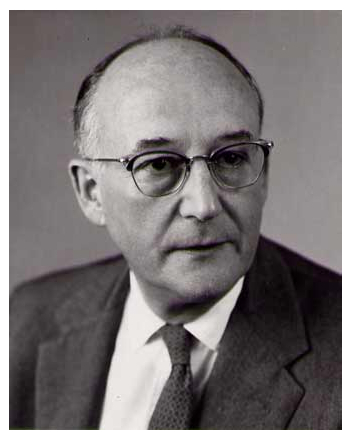
\includegraphics[scale=0.5]{images/morris.jpg}
  \caption{Charles William Morris (1901-1979)}
  \label{morris}
\end{figure}

One of the founders of semiotics, Charles William Morris, has identified the following important notions:

\begin{itemize}
\item \emph{Syntax}~--- relations between the signs of sign system themselves.
\item \emph{Semantics}~--- relations between a sign system and objects.
\item \emph{Pragmatics}~--- relations between a sign system and a person.
\end{itemize}

In a narrower context of programming languages syntax denotes the form of program representation, semantics~--- the ``meaning'' of programs, and pragmatics~---
the relation between programming language and developer. In our course we focus mainly on syntax and semantics, putting all pragmatics questions aside.

\section{Syntax}

Similarly to natural languages, the syntax of a programming language can be decomposed into a few levels (lexical structure, grammar, etc.) However,
unlike natural languages, which have been evolving more or less spontaneously, the syntax for a programming language is intelligently designed taking
into account a number of specific requirements; in particular, it is (as a rule) \emph{unabiguous} and allows for efficient analysis.

To illustrate the concept of programming language syntax consider the following simple snippet in \lang{C}:

\begin{figure}[h]
  \centering
  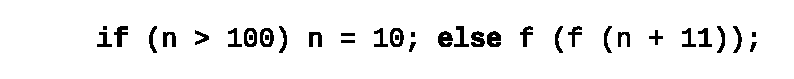
\includegraphics[scale=0.7]{images/01-01.eps}
\end{figure}

From the \emph{lexical} standpoint this fragment can be seen as a sequence of \emph{tokens} (a keyword, a delimiter, an identifier, a binary operator,
a decimal constant, etc.):

\begin{figure}[h]
  \centering
  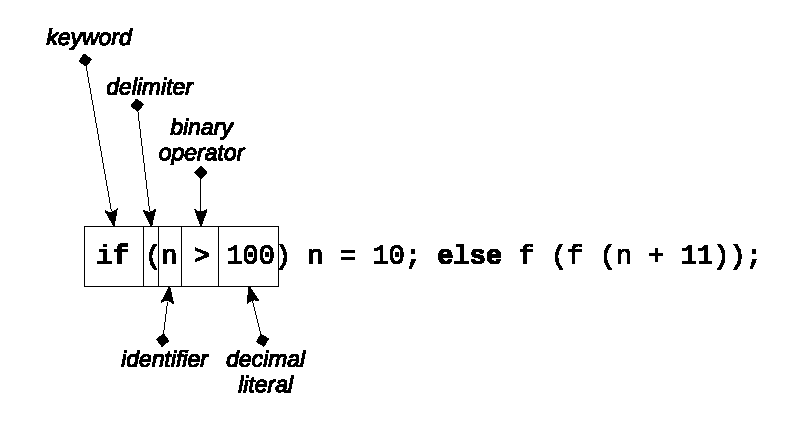
\includegraphics[scale=0.7]{images/01-02.eps}
\end{figure}

This sequence of tokens, in turn, is grouped into an hierarchy of syntactic constructs (in this case, expressions and operators):

\begin{figure}[h]
  \centering
  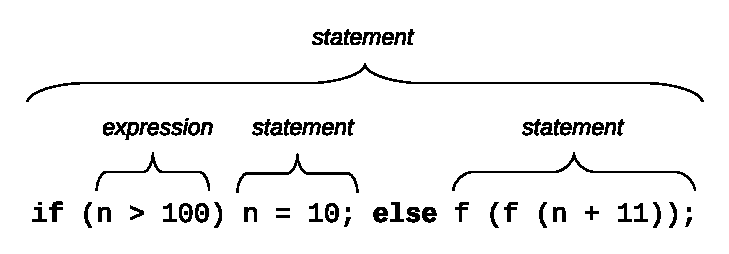
\includegraphics[scale=0.7]{images/01-03.eps}
\end{figure}

Natural languages, as a rule, are \emph{ambiguous}. Consider the following phrase: ``Entering the doors with pets hold them.`` Hold what? The doors or the pets?
In this case we encounter a \emph{global ambiguity} which cannot be resolved even taking into account the context. The only way to resolve it is to
rephrase (``Entering the doors hold your pets'' or ``Hold your pets while entering the doors''). The presence of such unresolvable ambiguities in a
programming language is inacceptable.

\section{Semantics}

The drastic difference between natural and programming languages manifests itself in a full bloom on the semantic level. Unlike natural languages,
for programming languages there are ways to formally specify their semantics and acquire a \emph{mathematically proven} results.

Why formal semantics matters? While in a common practice of using programming languages for application-level software we can rely on our vague, fuzzy
understanding of the meanings of their constructs, when we develop system-level programming \emph{tools}, in particular, compilers, this understanding
turns out to be insufficient. Imagine, for example, that we know that in some programming language expressions consist of variables, constant and four
arithmetic operators. Is this knowledge is complete?

Let us have the following expressions:

\begin{lstlisting}
   0*(x/0)
   1+x-x  
\end{lstlisting}      

What should be the results of their evaluation?

In the first sample, on one hand, the multiplication to zero always gives zero; on the other hand, the division by zero is undefined. So, would the result of
the expression be zero or undefined?

In the second sample, we add a value of \lstinline|x| to \lstinline|1| and immediately subtract it. On one hand this would give us \lstinline|1|; on the
other hand, the value of \lstinline|x| can be undefined, or adding \lstinline|x| to \lstinline|1| might lead to an overflow. So it remains unclear if we
can replace \lstinline|1+x-x| with \lstinline|1| while preserving the behaviour of the program in all cases.

Even if we cannot come up with definite oral answers to these questions we still can write programs using this language; after all, we always can
see what happens in each case if we have a compiler. But what should we do if our task is to implement the \emph{first} compiler for this language?
What happens if we ask a dozen of people to implement a dozen of compilers independently? Whould all these compilers agree in their semantics, or, perhaps, we
eventually will have a dozen of \emph{different} compilers since their authors have \emph{different} intuition? 

One may argue that all these samples come from a very rare and unrealistic use cases. Indeed, how often a new compiler is created, let alone a
dozen of those? And those snippets with ``murky'' semantics look like antipatterns: why on earth a sane developer whould write ``\lstinline|0*(x/0)|''
instead of ``\lstinline|0|'' or ``\lstinline|1+x-x|'' instead of ``\lstinline|1|''?

The answer, somewhat unexpected, is that actually all these cases are rather \emph{general} then exceptional. Of course, implementing a completely new compiler from scratch is not an
everyday task; however, at the same time programming languages and compilers are rarely developed ``once and for all''. As a rule, both languages
and their compilers evolve through time: new constructs are being added to languages, and new features are being implemented in compilers. Carrying out all of
these routine tasks require a strong semantic foundations. Besides this, compilers by no means are the only semantic-sensitive development instruments:
there is an abundance of other important tools like IDEs, model checkers, static analyzers, debuggers, profilers, etc., all of which have to interpret the
semantics of programs in a coherent way.

Then, not all programs are written directly by human beings. Actually, a fair share of them are generated by other tools, in particular, \emph{preprocessors}
or other \emph{metaprogramming} tools. The results of metaprogramming as a rule look exactly like the samples discussed above: they contain a lot
of vacuous use of constructs and programming language features, and it is \emph{expected} from the underlying compiler to clean up this mess
in a semantics-preserving manner.

Finally, for a compiler there is nothing ``weird'' in those code samples. The reason is simple: compilers do not have intuition. They just 
routinely convert program texts into executables no matter how weird they would look from a human being point of view. To illustrate this,
consider the following short program in \lang{C}: 

\begin{lstlisting}[language=cc]
m(f,a,s)char*s;
{char c;return f&1?a!=*s++?m(f,a,s):s[11]:f&2?a!=*s++?
1+m(f,a,s):1:f&4?a--?putchar(*s),m(f,a,s):a:f&8?*s?
m(8,32,(c=m(1,*s++,"Arjan Kenter. \no$../.\""),
m(4,m(2,*s++,"POCnWAUvBVxRsoqatKJurgXYyDQbzhLwkNjdMT"
"GeIScHFmpliZEf"),&c),s)):65:(m(8,34,"rgeQjPruaOnDaP"
"eWrAaPnPrCnOrPaPnPjPrCaPrPnPrPaOrvaPndeOrAnOrPnOrPn"
"OaPnPjPaOrPnPrPnPrPtPnPrAaPnBrnnsrnnBaPeOrCnPrOnCaP"
"nOaPnPjPtPnAaPnPrPnPrCaPnBrAnxrAnVePrCnBjPrOnvrCnxr"
"AnxrAnsrOnvjPrOnUrOnornnsrnnorOtCnCjPrCtPnCrnnirWtP"
"nCjPrCaPnOtPrCnErAnOjPrOnvtPnnrCnNrnnRePjPrPtnrUnnr"
"ntPnbtPrAaPnCrnnOrPjPrRtPnCaPrWtCnKtPnOtPrBnCjPronC"
"aPrVtPnOtOnAtnrxaPnCjPrqnnaPrtaOrsaPnCtPjPratPnnaPr"
"AaPnAaPtPnnaPrvaPnnjPrKtPnWaOrWtOnnaPnWaPrCaPnntOjP"
"rrtOnWanrOtPnCaPnBtCjPrYtOnUaOrPnVjPrwtnnxjPrMnBjPr"
"TnUjP"),0);}
main(){return m(0,75,"mIWltouQJGsBniKYvTxODAfbUcFzSp"
"MwNCHEgrdLaPkyVRjXeqZh");}
\end{lstlisting}

If you have any doubts if this is a valid \lang{C} program, compile and run it. \lang{C} is never considered as particularly hard to
understand or syntactically challenging (both arguable), yet the program presented is totally incomprehendible. Actually, it
was specifically designed to be such: there is a whole competition in writing \emph{obfuscated}
code\footnote{https://www.cise.ufl.edu/$\tilde\,$manuel/obfuscate/obfuscate.html}. For us, however, the important observation is that this
program no more obfuscated for a compiler as any other one. Our job as compiler implementors is to make them behave in such a way.


\section{The Essence of Translation}

\emph{Translation} is a syntactic transformation of programs in one language into (equivalent) programs into another.
The feasibility of fully automatic translation constituties a drastic difference between programming languages and natural ones.
Although natural language translation techniques and tools made a tremendous progress in a recent years the adequacy of the results
remains the matter of discusstion; and, anyway, this adequacy can not be mathematically proven. For compilers this problem
is essentially solved.

A compiler itself is not a magical creature~--- it is a \emph{program}, written, in turn, in some programming language. Thus, speaking
about compilation, we actually deal with \emph{three} languages:

\begin{figure}[h]
  \centering
  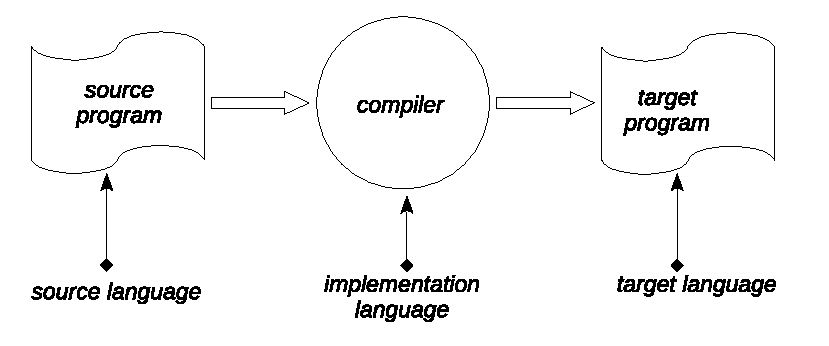
\includegraphics[scale=0.7]{images/01-04.eps}
\end{figure}

\begin{itemize}
\item The language in which the programs being compiled are written (\emph{source language}).
\item The language in which the programs being compiled are compiled (\emph{target language}).
\item The language in which the compiler from source to target language is written (\emph{compiler implementation language}).
\end{itemize}

\section{Translation Subspecies}

As you probably know, there is a subdivision of languages into high- and low-level. This subdivision is not absolute: for example,
\lang{Haskell} is considered by many as more high-level language than \lang{C}, which, in turn, is of higher level then \lang{Fortran}, etc.
As a rule, high-level languages are equipped with type systems, while low-level are not (but \lang{Scheme} is untyped while there 
exist typed assemblers). This coarse-grained classification of languages leads to a corresponding coarse-grained classification of
translators:

\begin{figure}[h]
  \centering
  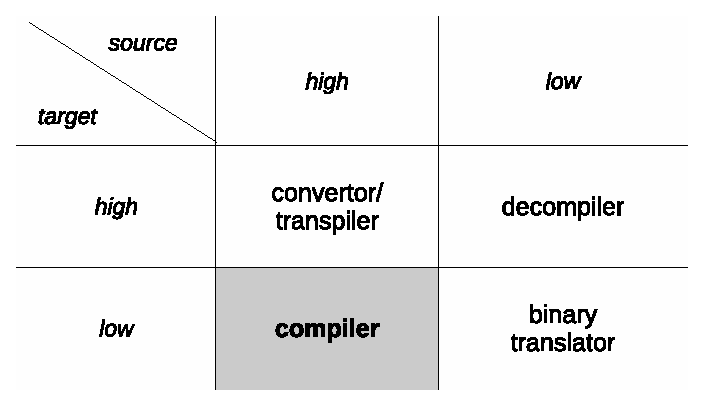
\includegraphics[scale=0.7]{images/01-05.eps}
\end{figure}

There is a somewhat common knowledge that among all these subspecies compilers are the most challenging to implement. While
we generally agree, it's worth mentioning that the other kinds of translators are not pieces of cakes at all: for example,
it is expeccted from a decompiler or convertor to properly utilize the abstractions of the target language, to produce a
human-readable maintanable results, etc.

\section{Environments, Runtime Support and\\
  Cross-Compilation}

Programs are rarely work in isolation; as a rule they rely on a certain environment: operation system, system- and user-level
libraries, etc. An important component of this environment is a \emph{runtime support library}. This library contains
an implementation of certain programming language constructs which are more beneficient to implement as a
library then to built in a compiler itself, for example, memory managements and synchronization primitives, etc. The
invocation of these primitives is generated by a compiler; as a rule, they can not be accessed from programs on the user level.
In contrast, \emph{standard library} contains an initial implementation of useful data structures and functions
in terms of the source programming language, for example, input-output functions, standard data types, collection implementations, etc.

Since compiler is a program itself, it also requires a certain environment, called \emph{compilation environment}.
On the other hand, the environment for which compiler generates its output is called \emph{target environment}. Usually these two
coinside~--- for example, out \lama compiler works under Linux on x86 processor, and generates programs which work
under Linux on x86.

However, in general case, compilation environment can be different from the target one. In this case the compiler is called
\emph{cross-compiler}. For example, we could rewrite our \lama compiler into a cross-one, which, still running on x86,
would generate code for ARM. 

A typical scenario for cross-compilation is \emph{bootstrapping} (see below) or the development of embedded systems when
the target platform is not enough performant/well-equipped to support the execution of a compiler.

\section{Bootstrapping}

An interesting (and practically important) operation involving compilers is their \emph{bootstrapping}. This term denotes the
implementation of a compiler in its own source languages (i.e. when implementation language coinsides with the source one).
The term itself originates from an idiom describing a process of pulling oneself up by the hooks on the back of their own
boots.

\begin{figure}[h]
  \centering
  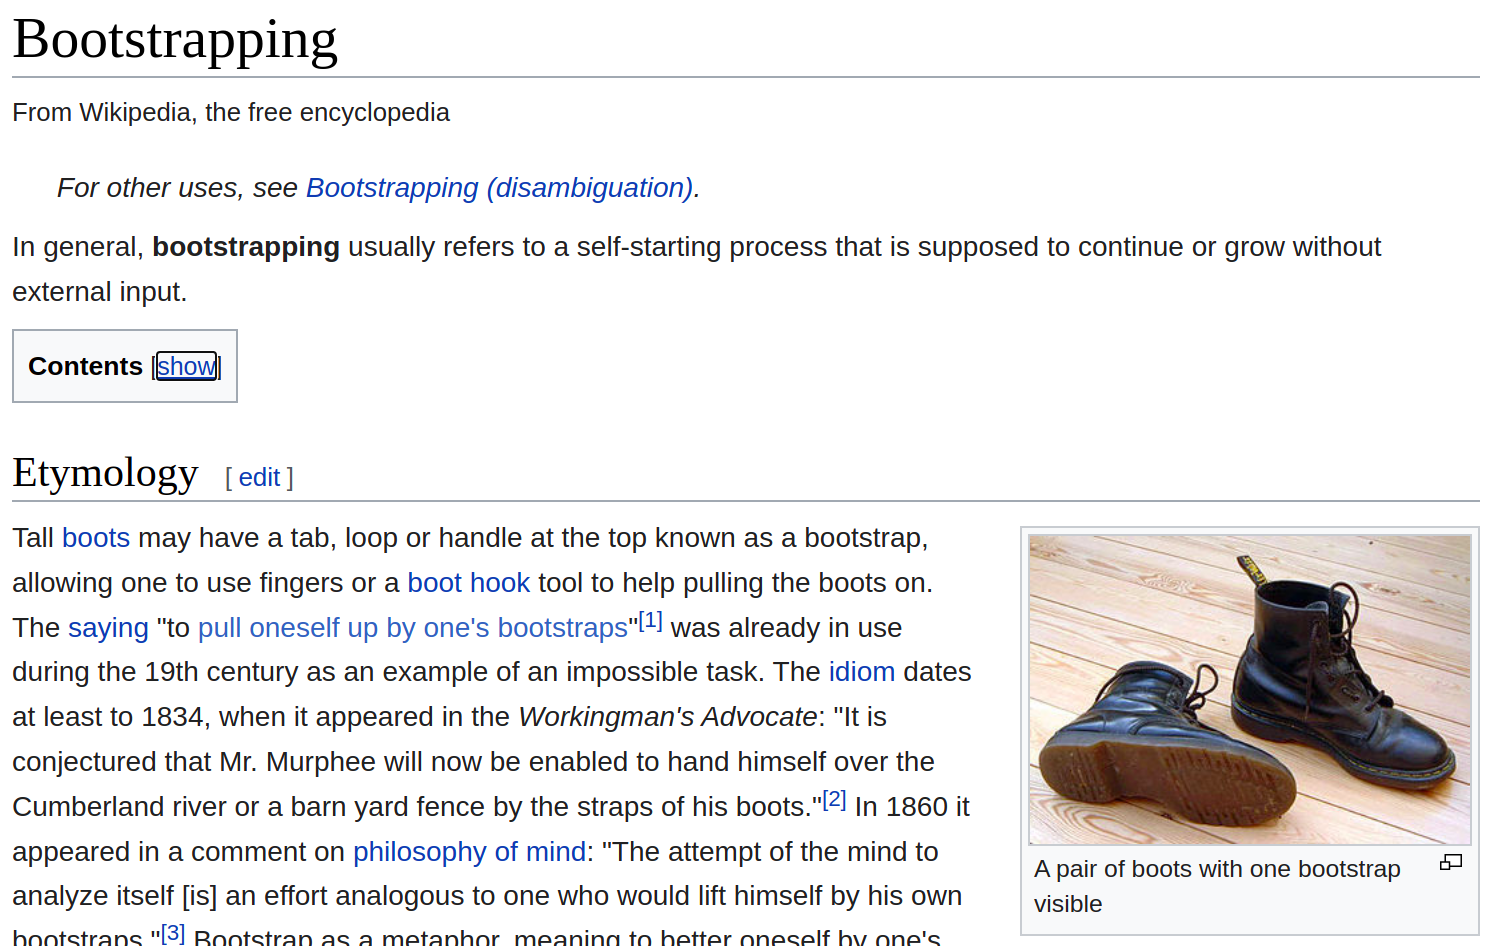
\includegraphics[scale=0.2]{images/bootstrapping.png}
\end{figure}

The bootstrapping of a compiler for a new language (for which no compiler yet exists) is compised of its implementation
in some other language and then rewriting it in this new language using just written compiler. For example, in such a way the \lama compiler was
acquired (\textbf{not really yet}): initially it was implemented in \lang{OCaml} and then reimplemented in
\lama itself.

If some compiler for the language of interest already exists, but works on some other platform, then it is possible for
implement a \emph{cross-compiler} which works on that platform but generates code for the platform of interest. Then
this compiler can be compiled by itself~--- this is the conventional way, for example, to port \sys{GCC} compilers
to other platforms.

Finally, if nothing useful exists beside the assembler for the platform of interest, then this assembler itself can be
used to implement a small subset of the desirable language; then this subset can be used to implement a wider subset, and so on.
This is how modern compiler/language zoo was built historically.

Compiler bootstrapping is an ideologically important step: first, it assesses the expressivenes of the language; second, ir witnesses the
maturity of the compiler, since for a new language its compiler, as a rule, is the first large and complex program.

\section{Complete vs. Partial Correctness}

Compiler (as any other translator) has to syntactically transform a program in one language into a program in another, preserving its semantics.
In practice, however there are some subtleties.

Let us have a program $\primi{p}$. We denote by

\[
x\xrightarrow{\displaystyle{\primi{p}}} y
\]

the fact that $\primi{p}$ on input $x$ terminates with the output $y$ (as we know, there may be two other outcomes: $\primi{p}$ crashes on input $x$ or
$\primi{p}$ loops forever on input $x$). 

Let us have a compiler, let $source$ be some source program, and let $target$ be a target program after the compilation.
We will say that a compiler is \emph{completely correct} iff for arbitrary $source$-$target$ pair and arbitrary
input-output pairs $x$ and $y$

\[
x\xrightarrow{\displaystyle{source}}y \Longleftrightarrow x\xrightarrow{\displaystyle{target}}y
\]

In other words, the behaviour of the source and compiled programs is indistinguishable: on the same input both either
terminate with the same results, or crash/loop.

Consider, however, the following simple program:

\begin{lstlisting}[language=cc]
   # include <stdio.h>

   static int d = 0;

   int main (int argc, char *argv[]) {
     int x;

     x = argc / d;
    
     return 255;
   }  
\end{lstlisting}

A brief analysis reveals that this program has to crash on each input. Indeed, the variable ``\lstinline[language=cc,basicstyle=\normalsize]|d|'' has initial value zero and cannot
be reassigned elsewhere (due to ``\lstinline[language=cc,basicstyle=\normalsize]|static|'' storage class), and division by zero gives a runtime error. We could, alternatively,
try to compile this program with ``\texttt{gcc -O0}'' command and see that it, indeed, crashes.

On the other hand, a more careful analysis shows that the value of the variable ``\lstinline[language=cc,basicstyle=\normalsize]|x|'', during the computation
of which the error occurs, actually is never used, so its computation can be completely omitted. And, indeed, if we compile this program with the command ``\texttt{gcc -O3}'',
it terminates successfully with return code 255! This is because the option ``\texttt{-O3}'' turns on the optimizations, and one of those~--- \emph{dead code elimination}~---
does exactly what we envisioned.

Thus, we can see that in practice target programs not always completely equivalent to the source ones: they can deliver some results on inputs, for which the source
ones loop or crash. This property is called \emph{partial correctness}, and can be formally specified as follows: for arbitrary input-output values $x$ and $y$, and for
arbitrary source and target programs $source$ and $target$

\[
x\xrightarrow{\displaystyle{source}}y \Longrightarrow x\xrightarrow{\displaystyle{target}}y
\]

This means, that when the source program terminates with a definite result, the target also does so with the same result; however, the target one can still deliver some output
values for inputs on which the source program is not defined. In other words, compilers are allowed to \emph{extend the domains} of programs they compile. The
majority of compilers (and other tools as well) are partially correct.

\section{Compiler Architecture}

The majority of real compilers share the same architectural features. They consist of a number of \emph{passes}, each of which
takes as input and returns as a result a certain \emph{intermediate represetation}, \emph{IR}, (not neccessarily the same) of a program
being compiled. The concrete set of these passes and concrete forms of intermediate representations vary from a compiler to a compiler,
but there are still some common representation which can be found throuhout various implementations: \emph{abstract syntax tree},
\emph{three-address code}, \emph{stack machine code}, \emph{static single assignment} (SSA), etc. Some of these forms of representation
will be utilized in our compiler, some others will be left out unused.

All the diversity of passes can be subdivided in a few categories.

\begin{figure}[h]
  \centering
  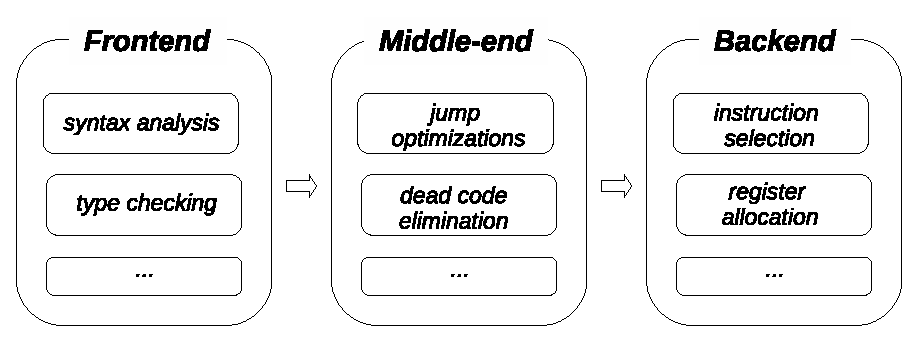
\includegraphics[scale=0.7]{images/01-06.eps}
\end{figure}

First, the \emph{frontend} of a compiler collects a number of \emph{analyzing} passes: syntax analysis, type inference/checking,
name resolution, etc.

Then, the \emph{backend} of a compiler contains code generation passes: instruction selection, register allocation,
instruction scheduing, low-level optimizations.

Finally, there can be \emph{middle-end}, which comprised of various machine-independent optimising passes such as
jump optimizations, dead code elimintation, loop invariant code motion, common subexpression elimination, etc.

Most compilers allow to peep on what's going on under the hood. For example, \texttt{GCC} accepts the
option \texttt{-ftime-report}, which makes it output the time taken by each pass performed. An example
of such an output is shown below:

\begin{scriptsize}
\begin{verbatim}
Execution times (seconds)
 phase setup             :   0.00 ( 0%) usr   0.00 ( 0%) sys   0.00 ( 0%) wall    1179 kB (25%) ggc
 phase parsing           :   0.03 (33%) usr   0.01 (100%) sys   0.04 (40%) wall    1197 kB (25%) ggc
 phase opt and generate  :   0.06 (67%) usr   0.00 ( 0%) sys   0.06 (60%) wall    2328 kB (49%) ggc
 callgraph optimization  :   0.01 (11%) usr   0.00 ( 0%) sys   0.00 ( 0%) wall       0 kB ( 0%) ggc
 cfg cleanup             :   0.00 ( 0%) usr   0.00 ( 0%) sys   0.01 (10%) wall       0 kB ( 0%) ggc
 trivially dead code     :   0.00 ( 0%) usr   0.00 ( 0%) sys   0.01 (10%) wall       0 kB ( 0%) ggc
 df reaching defs        :   0.01 (11%) usr   0.00 ( 0%) sys   0.00 ( 0%) wall       0 kB ( 0%) ggc
 alias analysis          :   0.01 (11%) usr   0.00 ( 0%) sys   0.00 ( 0%) wall      55 kB ( 1%) ggc
 preprocessing           :   0.00 ( 0%) usr   0.00 ( 0%) sys   0.01 (10%) wall     345 kB ( 7%) ggc
 lexical analysis        :   0.03 (33%) usr   0.01 (100%) sys   0.01 (10%) wall       0 kB ( 0%) ggc
 parser inl. func. body  :   0.00 ( 0%) usr   0.00 ( 0%) sys   0.02 (20%) wall      79 kB ( 2%) ggc
 dominator optimization  :   0.00 ( 0%) usr   0.00 ( 0%) sys   0.01 (10%) wall      45 kB ( 1%) ggc
 forward prop            :   0.01 (11%) usr   0.00 ( 0%) sys   0.00 ( 0%) wall      13 kB ( 0%) ggc
 loop init               :   0.02 (22%) usr   0.00 ( 0%) sys   0.01 (10%) wall     193 kB ( 4%) ggc
 loop fini               :   0.00 ( 0%) usr   0.00 ( 0%) sys   0.01 (10%) wall       0 kB ( 0%) ggc
 final                   :   0.00 ( 0%) usr   0.00 ( 0%) sys   0.01 (10%) wall      48 kB ( 1%) ggc
 TOTAL                 :   0.09             0.01             0.10               4714 kB
\end{verbatim}
\end{scriptsize}

\begin{figure}[t]
  \centering
  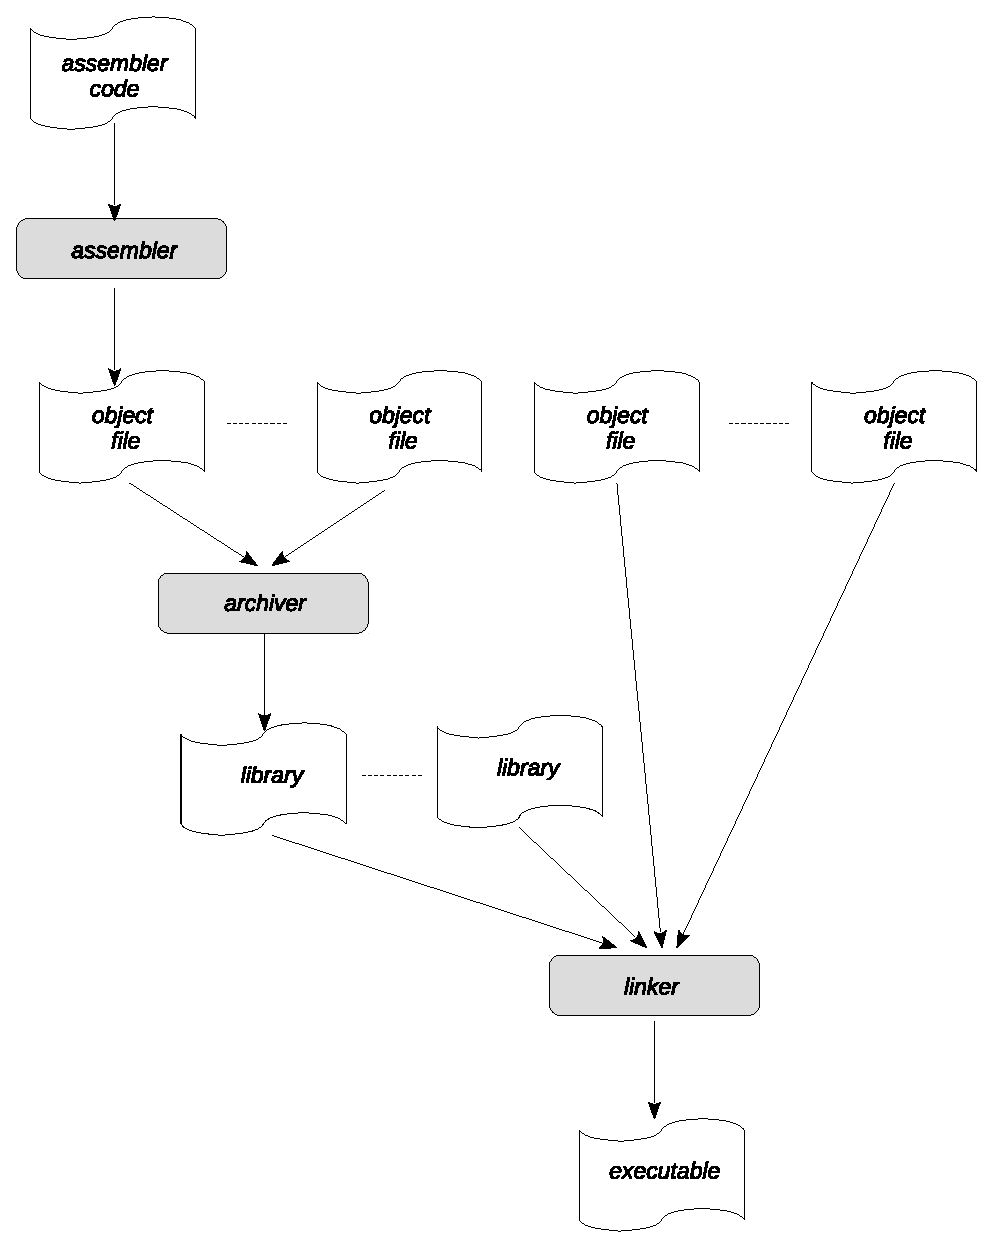
\includegraphics[scale=0.7]{images/01-09.eps}
  \caption{Toolchain}
  \label{toolchain}
\end{figure}

\section{Beyond Compilers}

While compilers, indeed, transform source programs to machine code, the code they output, as a rule, cannot be directly run on hardware.
The reason is that it still contains certain abstractions the hardware cannot deal with. In particular, compilers usually generate
assembler code with \emph{symbolic names}. This approach plays an important role in supporting \emph{separate compilation}~--- a
feature which allows to combine programs from a number of precompiled modules. The majority of application programs
make use of various libraries; as a rule, the source code of these libraries is not compiled alongside with the application itself, but
\emph{linked} at post-compilation time, thus greatly reducing the time required for build. To make it possible, compilers
produce not ready-to-run binary code, but so-called \emph{object files} which, besides machine code, contain supplementary
\emph{metadata} to make linking possible. Thus, on the way to the real executable binary the output which compilers provide
is transformed again a number of times.

In the most general case, the compiler generates a textual assembler program. Then the following tools can be used:

\FloatBarrier

\begin{itemize}
\item \emph{assembler} which reads assembler programs and outputs object files;
\item \emph{archiever/librarian} which combines multiple object files into one archive/library file;
\item \emph{linker} which combines multiple object and library files into one executable.
\end{itemize}

These tools together with a compiler form so-called \emph{toolchain} (Fig.~\ref{toolchain}). When a new processor comes to market it is expected from
the vendor to supply a conventional toolchain for the developers. In \sys{Unix}-like systems the conventional
toolchain consists of separate programs \prog{cpp} (\lang{C} preprocessor), \prog{cc} (\lang{C} compiler),
\prog{as} (assembler), \prog{ld} (linker) and \prog{ar} (archiever). \sys{GCC} compiler implements only two first
of these components~--- \prog{cpp} and \prog{cc},~--- and invokes others to complete the compilation process
depending on what options were specified by users. The top-level program \prog{gcc} itself is just a \emph{driver}
which controls the execution of other tools of the toolchain. 

\section{The \lama Compiler}

Now, when we discussed a little bit how compilers work, let's have a look at \lama compiler, which will be our main
tool throuhgout the course, and which we will be implementing.

The \lama compiler is organized much simpler than the majority of industrial-tier compilers like \texttt{GCC}, which we already
mentioned multiple times (see Fig.~\ref{lama-comp}).

\begin{figure}[t]
  \centering
  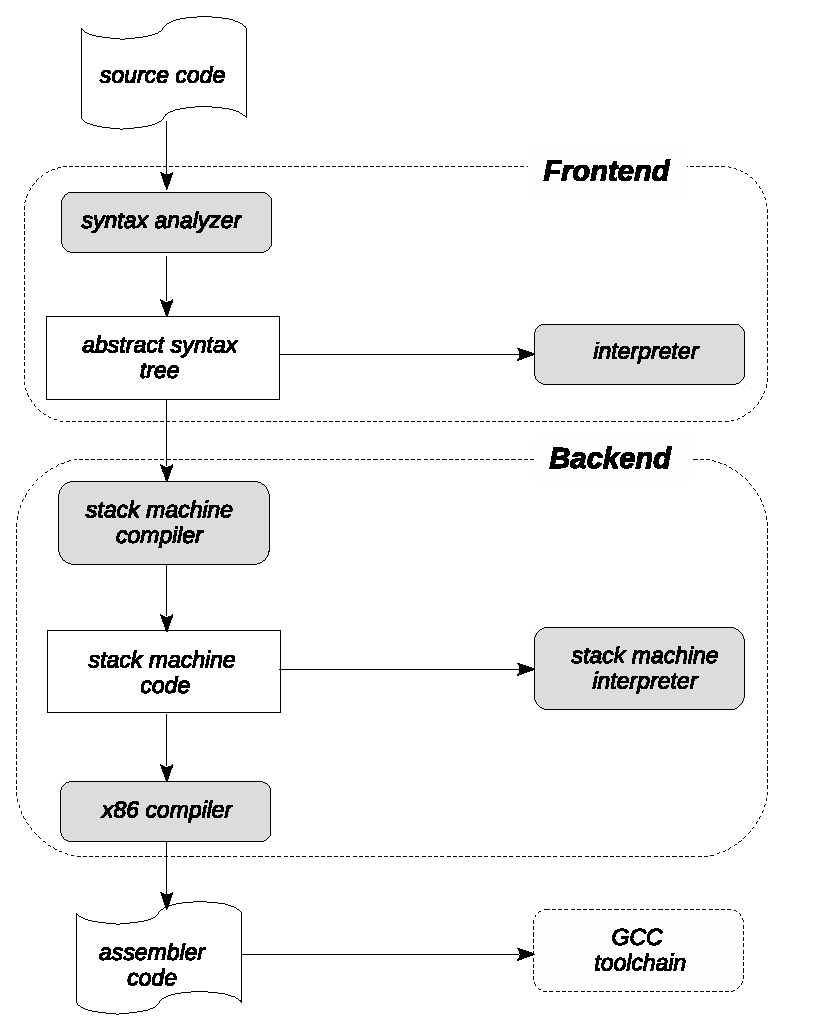
\includegraphics[scale=0.7]{images/01-07.eps}
  \caption{The Structure of \lama Compiler}
  \label{lama-comp}
\end{figure}

The source file with a \lama program is parsed by a syntax analyser which converts it into an
abstract syntax tree, or AST. An example of a program and its AST (actually, an \emph{HTML-rendering}
of its AST) is shown below:

\begin{tabular}{m{5cm}m{5cm}}
  \begin{lstlisting}[basicstyle=\small]
 printf ("Hello, world!\n")
  \end{lstlisting} &
  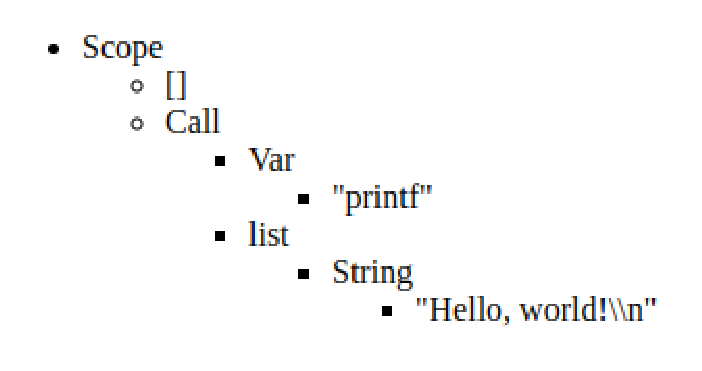
\includegraphics[scale=0.55]{images/01-08.eps}
\end{tabular}

AST is one of the most important program representations, and its use in compilers and other
tools is ubiquitious. 

The next component, which is rarely implemented in real-world compilers, is a source-level \emph{interpreter}. We
consider this object in details later, for now it is sufficient to know that interpreter is a component which
directly runs a program in some representation~--- in our case, in the form of AST,~--- according to the semantics of the language. 
The presence of interpreter plays an important role from both educational and technological standpoints. First,
the implementation of interpreter facilitates the internalization of formal semantics description method which
we use, namely~--- big-step operational semantics. Next, it allows to find and eiminate some errors 
at early stage. The implementation of interpreter is rather a simple task, and it is advantageous to be capable of running program
at early stages of compiler implementation.

Then, there is a compiler of AST into \emph{stack machine} code. This machine resembles a simplified model of
actual hardware processor; thus, on one hand, to generate stack machine code a similar set of tasks has to be
solved; on the other, these solutions are a bit simpler than for an actual hardware. For our example
program the corresponding stack machine code looks like

\begin{lstlisting}[language=plain,basicstyle=\small]
    LABEL ("main")
    BEGIN ("main", 2, 0, [], [], [])
    STRING ("Hello, world!\\n")
    CALL ("Lprintf", 1, false)
    END      
\end{lstlisting}

Generated stack machine code can then be run on the \emph{stack machine interpreter}. Similarly to source-level
interpreter case, the capability to run stack machine code makes it possible to develop and debug stack
machine compiler in isolation.

Finally, the last component of the compiler is code generator for \texttt{x86} processor which
transforms stack machine code into \texttt{x86} assembler program; this program is then passed to
the \textsc{GCC} infrastructure to be finally transformed into an object module. An example of
\texttt{x86} assembler listing for our example program is shown below:

\begin{lstlisting}[language=plain,basicstyle=\small]
             .globl	main
             .data
    string_0:.string "Hello, world!\n"
    main:
    # BEGIN ("main", 2, 0, [], [], []) / 
    # STRING ("Hello, world!\\n") / 
             movl	$string_0,	%ebx
	     pushl	%ebx
	     call	Bstring
	     addl	$4,	%esp
	     movl	%eax,	%ebx
    # CALL ("Lprintf", 1, false) / 
	     pushl	%ebx
	     call	Lprintf
	     addl	$4,	%esp
	     movl	%eax,	%ebx
    # END / 
	     movl	%ebx,	%eax
    Lmain_epilogue:
             movl	%ebp,	%esp
	     popl	%ebp
	     xorl	%eax,	%eax
	     ret
\end{lstlisting}

Thus, from the architectural point of view, syntax analyser constitutes a fronted, while compilers for
stack machine and \texttt{x86}~--- a backend.


\chapter{Semantics and Interpreters}

In this section we set the foundations for formal semantics which will be used in the rest of the course. We also discuss the
relation between programs and their representation in a concrete data domain, introduce the notion of interpreter and
consider some sample languages, their semantics and techniques for interpreter implementations.

\section{Languages and Semantics}

We consider programming language $\mathcal L$ as a (countable) set of programs

\[
\mathcal{L}=\{\primi{p}_1,\,\primi{p}_2,\dots\}
\]

To give a \emph{semantics} for the language $\mathcal L$ is to specify two objects:

\begin{itemize}
\item a \emph{semantic domain} $\mathcal D$;
\item a \emph{total} mapping $\sembr{\bullet}^\ph_{\mathcal L} : \mathcal L \to \mathcal D$.
\end{itemize}

Thus, for a program

\[
\primi{p}\in\mathcal L
\]

its semantics is just a

\[
\sembr{\primi{p}}^\ph_{\mathcal L}\in\mathcal D
\]

When the language is easily deducible from the context we will omit the subscript and write simply $\sembr{\bullet}$.

By claiming the totality of $\sembr{\bullet}$ we
make sure that any program has some semantics. The nature of semantic domain $\mathcal D$ essentially defines the nature of $\sembr{\bullet}_{\mathcal L}$;
for example, we can set

\[
\mathcal D=\{\Cat\}
\]

and (the only choice)

\[
\sembr{\primi{p}}=\Cat
\]

for every $\primi{p}\in\mathcal L$. We admit that this particular
semantics might not be very useful (this, however, depends on the nature of $\mathcal L$), but the important observations are that

\begin{itemize}
\item the choice of $\mathcal D$ has to be made;
\item there might be (and, \emph{as a rule}, are) multiple semantics for a given language.
\end{itemize}

These various semantics for a language may reflect its various properties (and we will see some of those in a little while); however, as a rule, one particular
semantics is chosen as the ``standard'' one.

\section{Data Domain}

If we speak of a general-purpose programming language and interested in its execution semantics then, probably, we may consider choosing the semantic domain
to be the set of all \emph{partially-recursive} functions and $\sembr{p}$ to be the function $p$ evaluates. This choice, however, would be too high-level and
abstract for our purposes.

To be more concrete, we first choose a \emph{data domain} $\mathfrak D$ to be the set of all reasonable data values the programs can take as inputs and
produce as outputs; then the semantic domain for executable semantics would be

\[
\mathcal{D}:\mathfrak{D}\to\mathfrak{D}
\]

Thus, executable semantics maps programs to data-processing functions.

In order to make further progress we stipulate the following properties of the data domain. First, we require its \emph{closedness under product}:

\[
\mathfrak{D}\times\mathfrak{D}\subset\mathfrak{D}
\]

In other words, $\mathfrak{D}$ contains all pairs, triples, etc. of its values.

The next requirement follows from out intention to make \emph{metaprogramming} possible. In short, the idea behind metaprogramming is
to use \emph{programs} as \emph{data}. Indeed, all programming tools follow this approach: a compiler takes a program as input and
returns (another) program as output, etc. This can be done only if programs can be \emph{encoded} somehow in the data domain. We
consider some concrete encodings, using \lama data domain later; for now we assume that for arbitrary programming language $\mathcal{L}$
the set $\mathfrak{D}$ contains the \emph{representations}
of all programs in $\mathcal{L}$:

\[
\forall \mathcal{L}\; .\; \mathcal{L}\subset\mathfrak{D}
\]

We agreed above to consider programming languages as sets of programs; we could, equivalently, consider them as sets of \emph{representations} of
programs in some universal data domain. Since the correspondence between programs and their representations is one-to-one this convention would
not hinder any follow-up reasonings. From now on we will not distinguish programs (abstract objects) from their representations (concrete objects)
in $\mathfrak{D}$. Note, there can be multiple representations within one data domain, but all of them are ``equivalent'' in the sense that
each pair of them admits an unambiguous conversions in both directions.

\section{Semantic Properties}

Let us have a language $\mathcal{L}$ and its \emph{two} semantics

\[
\begin{array}{rcl}
    \sembr{\bullet}^\ph & : & \mathcal{L} \to \mathcal{D}\\
  \sembr{\bullet}^\prime & : & \mathcal{L} \to \mathcal{D}
\end{array}
\]

with the \emph{same} semantic domain. We say that these semantics are \emph{equivalent} if and only if for arbitrary program $\primi{p}\in\mathcal{L}$

\[
\sembr{\primi{p}}^\ph=\sembr{\primi{p}}^\prime
\]

In other words, equivalent semantics assign to each program in the language the same element of semantic domain. A question might arise why would we
need two equivalent semantics; wouldn't the single one be sufficient? The answer is that there are multiple ways of
describing semantics, and these different ways have different properties which make them preferable in different settings. Sometimes it is desirable to
reformulate the semantics in different terms. By proving the equivalence between the two we can justify that we still deal with the language with the same
semantic properties.

Note, when the semantic domain is domain of functions $\mathfrak{D}\to\mathfrak{D}$, the equation above denotes the equality of functions: for
arbitrary $x, y\in\mathfrak{D}$

\[
\sembr{\primi{p}}^\prime\,x=y \Leftrightarrow \sembr{\primi{p}}\,x=y
\]

In other words, in both semantics $\primi{p}$ is defined on exactly the same inputs and for each of these inputs it provides the same outputs.

Another important property is \emph{equivalence of programs} within the same semantics. We say that $\primi{p}_1$ is (semantically) equivalent to $\primi{p}_2$ if
and only if

\[
\sembr{\primi{p}_1}=\sembr{\primi{p}_2}
\]

Thus, equivalent programs have the same semantics. The equivalence of \emph{different} programs within the same semantics plays a crucial
role in justifying the correctness of program transformations. Let us have some transformation of programs into programs:

\[
f : \mathcal{L}\to\mathcal{L}
\]

We say that $f$ is \emph{semantically correct} if and only if for all programs $\primi{p}$

\[
\sembr{f\,(\primi{p})}=\sembr{\primi{p}}
\]

Thus, equivalent transformations do not change the semantics of programs; they can, however, change other their properties.

When the semantic domain is domain of functions, the equation above, again, denotes the equality of functions; additionally,
the following important notion can be introduced in this case. We say that $f$ is \emph{partially correct} if and only if
for all programs $\primi{p}$ and all $x, y\in\mathfrak{D}$

\[
\sembr{\primi{p}}\,x=y\Rightarrow\sembr{f\,(\primi{p})}\,x=y
\]

The difference between correctness and partial correctness is that in the former case the programs are defined for exactly the same inputs,
while in the latter the transformed program can be defined even if the original one in not. To some extent this is how
optimizing transformations work, as we've seen in the previous chapter.

Finally, there can be transformations between \emph{different} languages with the \emph{same} semantic domain. Let us have two languages $\mathcal{L}$ and $\mathcal{M}$
and let their semantics be

\[
\begin{array}{rcl}
  \sembr{\bullet}^\ph_\mathcal{L} & : & \mathcal{L}\to\mathcal{D}\\
  \sembr{\bullet}^\ph_\mathcal{M} & : & \mathcal{M}\to\mathcal{D}
\end{array}
\]

We say that a transformation

\[
f : \mathcal{L}\to\mathcal{M}
\]

is \emph{semantically correct} if and only if for all programs $\primi{p}$

\[
\sembr{\primi{p}}^\ph_\mathcal{M}=\sembr{f\,(\primi{p})}^\ph_\mathcal{L}
\]

And, again, when $\mathcal{D}$ is a domain of functions the equation above denotes the equality of functions, and the notion of
partial correctness arises. One example of transformation between languages is compilation; as we already know, compilers as a rule
are partially correct.


\section{Interpreters, Compilers, Specializers}

We already mentioned compilation as a syntactic transformation from one language to another; we also
talked of compilers as programs which implement compilation. Here we consider them and some other useful
transformations in the form of programs in more details.

Let $\mathcal{L}$ and $\mathcal{M}$ be two languages, and

\[
\begin{array}{rcl}
\sembr{\bullet}^\ph_{\mathcal L} & : & \mathcal{L} \to \mathfrak{D} \to \mathfrak{D}\\
\sembr{\bullet}^\ph_{\mathcal M} & : & \mathcal{M} \to \mathfrak{D} \to \mathfrak{D}
\end{array}
\]

--- their semantics. An \emph{interpreter} for language $\mathcal{L}$, written in language $\mathcal{M}$, is a program $\Int{L}{M}\in\mathcal{M}$, such that for each
program $\primi{p}^\ph_\mathcal{L}\in\mathcal{L}$ and each data value $x\in\mathfrak{D}$

\[
\sembr{\Int{L}{M}}^\ph_\mathcal{M}\,(\primi{p}^\ph_\mathcal{L}\times x) = \sembr{\primi{p}^\ph_\mathcal{L}}^\ph_\mathcal{L}\,(x)\eqno{(\star)}
\]

To some extent an interpreter \emph{implements} the semantics of a programming language: given a program and its input it provides exactly the same result
this program calculates. Of course there can be many interpreters for a given pair of languages; any program $\primi{i}^\ph_\mathcal{M}$ satisfying equation $(\star)$,
e.g. such than

\[
\forall \primi{p}^\ph_\mathcal{L},\,x\in\mathfrak{D}\,.\,\sembr{\primi{i}^\ph_\mathcal{M}}^\ph_\mathcal{M}\,(\primi{p}^\ph_\mathcal{L}\times x)=\sembr{\primi{p}^\ph_\mathcal{L}}^\ph_\mathcal{L}\,(x)
\]

is an interpreter.

A particular interesting kind of interpreter is \emph{self}-interpreter $\Int{L}{L}$, i.e. an interpreter which interprets the language of its own implementation.
In the computability theory such interpreters are known under the name ``\emph{universal functions}'', and it is proven than universal functions exist for
all Turing-complete languages.

Another interesting program is, of course, compiler. Given languages $\mathcal{L}$, $\mathcal{M}$, and $\mathcal{N}$, a compiler from
$\mathcal L$ to $\mathcal N$, written in a language $\mathcal M$, is a program $\Comp{L}{N}{M}\in\mathcal M$ such that
for all programs $\primi{p}^\ph_\mathcal{L}\in\mathcal L$ and all input data values $x\in\mathfrak{D}$ the following equation holds:

\[
\sembr{\sembr{\Comp{L}{N}{M}}^\ph_\mathcal{M}\,(\primi{p}^\ph_\mathcal{L})}^\ph_\mathcal{N}\,(x) = \sembr{\primi{p}^\ph_\mathcal{L}}^\ph_\mathcal{L}\,(x)\eqno{(\star\star)}
\]

Indeed, a compiler takes a program representation $\primi{p}^\ph_\mathcal{L}$ as input and produces another program, $\sembr{\Comp{L}{N}{M}}^\ph_\mathcal{M}\,(\primi{p}^\ph_\mathcal{L})$,
this time in the language $\mathcal{N}$, which gives exactly the same result as $\primi{p}^\ph_\mathcal{L}$ for any input $x$. And, again, any program $\primi{c}^\ph_\mathcal{M}$ satisfying
the equation $(\star\star)$ is a compiler.

Finally, there can be a program called \emph{specializer} $\Spec{L}{M}$, written in a language $\mathcal M$ for a language $\mathcal L$, such that for
all programs $\primi{p}^\ph_\mathcal{L}\in\mathcal L$ and all data values $x, y\in\mathfrak D$

\[
\sembr{\sembr{\Spec{L}{M}}^\ph_\mathcal{M}\,(\primi{p}^\ph_\mathcal{L}\times x)}^\ph_\mathcal{L}\,(y)=\sembr{\primi{p}^\ph_\mathcal{L}}^\ph_\mathcal{L}\,(x\times y)\eqno{(\star\star\star)}
\]

Informally, a specializer takes as input a program $\primi{p}^\ph_\mathcal{L}$ and \emph{one} of its inputs $x$ and builds a program in the same language $\mathcal L$ which
takes $y$~--- the remaining inputs of $\primi{p}^\ph_\mathcal{L}$,~--- and provides exactly the same result as $\primi{p}^\ph_\mathcal{L}$ for both $x$ and $y$. The existence of specializers is,
again, guaranteed by the computability theory (\emph{Kleene $s$-$m$-$n$--theorem}).

%It's worth discussing why (and, actually, when) these programs exist. Obviously, if both $\mathcal{L}$ and $\mathcal{M}$ are Turing-complete, there exist
%both $\Int{L}{M}$ and $\Int{M}{L}$ (why?).

\section{Futamura Projections}

We now study an few elegant theoretical constructs which connect together the notions of interpreters, compilers and specializers. To simplify the presentation we
introduce the following denotation

\[
p^\ph_\mathcal{L}=\sembr{\primi{p}^\ph_\mathcal{L}}^\ph_\mathcal{L}
\]

for a program $\primi{p}^\ph_\mathcal{L}$. Thus, while $\primi{p}^\ph_\mathcal{L}$ is a program in a language $\mathcal{L}$ (i.e. a syntactic object), $p^\ph_\mathcal{L}$ is
its semantics (a function in the data domain).

Our first step is to apply a specializer $\Spec{L}{M}$ to some interpreter $\Int{N}{L}$ and some program $\primi{p}^\ph_\mathcal{N}$ it can interpret:

\[
\sembr{\underline{\SpecS{L}{M}\,(\Int{N}{L}\times \primi{p}^\ph_\mathcal{N})}}^\ph_\mathcal{L}\,(x)=\IntS{N}{L}\,(\primi{p}^\ph_\mathcal{N}\times x)=\sembr{\underline{\primi{p}^\ph_\mathcal{N}}}^\ph_\mathcal{N}\,(x)\eqno{(I)}
\]

The first equality follows immediately from $(\star\star\star)$ while the second~--- immediately from $(\star)$. Let's now look at the underlined parts. The \emph{right} one is, obviously,
$\primi{p}^\ph_\mathcal{N}$, a program in the language $\mathcal{N}$. The \emph{left} one is some program in the language $\mathcal{L}$. The equation itself states that the semantic of these
two programs give the same value for every input $x$. In other words, these two programs are equivalent. This is the first Futamura projection:

\begin{quote}
  \emph{The specialization of an interpreter for a program gives the representation of this program in the language of interpreter implementation.}
\end{quote}

Next, let's specialize a specializer for an interpreter:

\begin{multline*}
  \sembr{\sembr{\underline{\SpecS{M}{K}\,(\Spec{L}{M}\times\Int{N}{L})}}^\ph_\mathcal{K}\,(\primi{p}^\ph_\mathcal{N})}^\ph_\mathcal{L}\,(x)=\\
  \sembr{\SpecS{L}{M}\,(\Int{N}{L}\times \primi{p}^\ph_\mathcal{N})}^\ph_\mathcal{L}\,(x)=
  \sembr{\primi{p}^\ph_\mathcal{N}}^\ph_\mathcal{N}\,(x)\tag{II}
\end{multline*}

The first equation, again, immediately follows from $(\star\star\star)$, while the second~--- from $(I)$. If to look at the underlined part long enough, it becomes
evident that it is a program in the language $\mathcal{M}$ which satisfies the equation $(\star\star)$, i.e. a compiler $\Comp{N}{L}{M}$. This is a second Futamura projection:

\begin{quote}
  \emph{The specialization of a specializer to an interpreter gives a compiler from the interpreting language to the language of interpreter implementation.}
\end{quote}

Finally, we can specialize a specializer to a specializer:

\[
  \sembr{\SpecS{K}{T}\,(\Spec{M}{K}\times\Spec{L}{M})}^\ph_\mathcal{T}\,(\Int{N}{L})=\SpecS{M}{K}\,(\Spec{L}{M}\times\Int{N}{L})\eqno{(III)}
\]

The equation immediately follows from $(\star\star)$; its right part, according to $(II)$, is $\Comp{N}{L}{M}$. This is the
third Futamura projection:

\begin{quote}
  \emph{The specialization of a specializer to a specializer gives a compiler generator which for an interpreter generates a compiler from
  the interpreting language to the language of interpreter implementation.}
\end{quote}

Futamura projections are named after Y.Futamura, who described the first two of them in the beginning of 1970s. All three
projections were independently discovered by V.Turchin and A.Ershov, who gave them their current name.

The beauty of Futamura projections is that they give a rather simple equations for rather complex tools like compilers and compiler generators.
However, this immediately raises a question if one can indeed acquire these tools using such a high-level description.

Let's assume that we are going to use Futamura projections to implement a compiler from \lama to \texttt{x86}. Then we, first, need an interpreter
$\Int{\mbox{\lama}}{\mbox{\texttt{x86}}}$ for \lama written in \texttt{x86} assembler. The task of implementing such an interpreter, while involving
some low-level programming, does not look very challenging. Then, we need a specializer $\Spec{\mbox{\texttt{x86}}}{\mathcal{L}}$ for \texttt{x86}
assembler written in some language $\mathcal{L}$, not necessarily \lama. We can choose any suitable language for this purpose. Having both at
hands, we will be able to compile \lama-programs to \texttt{x86} code using the first Futamura projection:

\[
\SpecS{\mbox{\texttt{x86}}}{\mathcal{L}}\,(\Int{\mbox{\lama}}{\mbox{\texttt{x86}}}\times \primi{p}^\ph_{\mbox{\lama}})=\primi{p}^\ph_{\mbox{\texttt{x86}}}
\]


And here comes the hard part: the simplest possible specializer (for example, that guaranteed by the $s$-$m$-$n$--theorem) would produce a very
poor machine code; it would, in fact, just link the interpreter with the program, which invalidates the very idea of compilation. In order to
acquire a decent result, the specializer has to be non-trivial. The task of developing a non-trivial specializer even for the first Futamura
projection is non-trivial as well; nevertheless there are frameworks where this task is solved. For example, \texttt{GraalVM} uses the first Futamura projection
as a tool for language bootstrapping.

If we move higher in the Futamura projection hierarchy we would need at least one additional specializer $\Spec{L}{L}$, this time
for the language $\mathcal{L}$; it can be written in the $\mathcal{L}$ as well. This specializer has to be even more advanced than
$\Spec{\mbox{\texttt{x86}}}{\mathcal{L}}$ since we expect it to decently specialize more complicated program, than interpreters.

Finally, for the third Futamura projection we need even more advanced specializer since it has to be capable of decently specialize specializer for a
specializer. Note, is the third Futamura projections the last two specializers need not necessarily be the same programs, but it is very
appealing from both scientific and aesthetic standpoints to have the single, \emph{self-applicable}, specializer.

Thus, using Futamura projections beyond the first one in practice is still a hard venture. In the middle of 1980s all three projections were
implemented by the group led by N.Jones, but this was rather a proof-of-concept than a working industrial technology.

\chapter{Straight Line Programs}

In this chapter we introduce the language of \emph{straight line} programs which can be considered as a smallest
non-trivial subset of \lama. In this subset all programs are executed sequentially statement by statement with
no branching. Thus, any program either comes to an end or stops due to an error, but cannot loop forever. We
use this simple language to showcase all the ingredients of our approach to language description: abstract and
concrete syntax specification, denotational and operational semantics, etc. We also introduce some components of
the compiler we will be working on: source-level interpreter, stack machine compiler and interpreter, and
\texttt{x86} code generator.

\begin{figure}[t]
  \centering
  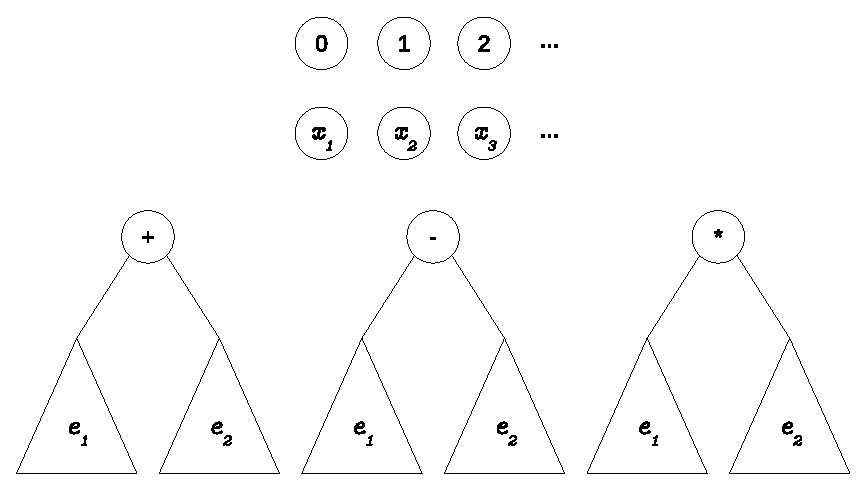
\includegraphics[scale=0.7]{images/02-01.eps}
  \caption{Abstract Syntax for Expressions}
  \label{expression-syntax}
\end{figure}

\section{Expressions}


Syntactically, our language encorporates two \emph{syntactic categories}: expressions and statements. We start from describing
so-called \emph{abstract syntax} for the expression category. We consider a countable set of \emph{variables}

\[
\mathscr{X}=\{x_1,\,x_2,\,\dots\}
\]

and a set of \emph{binary operators}

\[
\otimes= \{+,\, -,\, \times,\, /,\, \%,\, <,\, \le,\, >,\, \ge,\, =,\,\ne,\, \vee,\, \wedge\}
\]

which contains all thirteen built-in \lama operators. Then, the category of expressions $\mathscr{E}$ can be defined by
the following recursive scheme:

\[
\begin{array}{rcl}
  \mathscr{E} & = & \mathscr{X} \\
              &   & \mathbb{N} \\
              &   & \mathscr{E}\otimes\mathscr{E}
\end{array}
\]

This scheme defines a countable set of \emph{labeled ordered trees} of finite height: each node of such a tree is labeled, and for any node the order
of its immediate subtrees is essential. The simplest trees of this form are just leaves labeled with either variables or natural numbers; we simply
write $\mathscr{X}$ or $\mathbb{N}$ in the first two lines of definition of $\mathscr{E}$, but actually we mean tree nodes \emph{labeled} by the symbols of
these sets. As for the third line, it stipulates that for arbitrary two expressions $e_1,\,e_2\in\mathscr{E}$ a tree with a root labeled with any symbol
from $\otimes$ and immediate subtress $e_1$ and $e_2$ is also expression (see Fig.~\ref{expression-syntax}).

We call this definition \emph{abstract} syntax because it describes nothing more than a subordination between elementary constructs. In order to represent
expressions in some medium, however, we need \emph{concrete} syntax; it is easy to anticipate that there can be multiple concrete syntaxes for given
abstract one. In Fig.~\ref{expression-concrete} we give some examples of those for expressions: the first (\emph{a}) consists of graphical elements such as
circles, lines, texts, etc. Another one (\emph{b}) is the familiar \emph{infix notation} which includes numbers, letters, binary
operators and brackets. Yet another (but by no means the last one) is \emph{reverse Polish notation} (\emph{c}), in which binary operators are
put \emph{after} the operands they connect. In what follows we will stick with infix notation.

\begin{figure}[t]
  \centering
  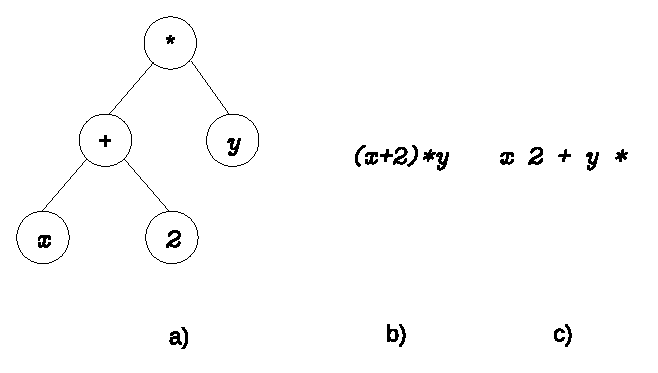
\includegraphics[scale=0.7]{images/02-02.eps}
  \caption{Various Concrete Syntaxes for Expression Language}
  \label{expression-concrete}
\end{figure}

Now we need to define the semantic domain for the semantics of expressions. We already hinted that this domain should be shaped like a set of some
data processing functions $\mathfrak{D}\to\mathfrak{D}$; however, we need to be more specific.

As we deal with arithmetic expressions it is rather natural to expect that the results of their evaluation are interger values, i.e. $\mathbb{Z}$ (as we agreed
earlier, we assume $\mathbb{Z}\subset\mathfrak{D}$); on the other hand, the value of an expression depends on the values of variables it contains. We can
encode these values as a \emph{state}~--- a function which maps variables to integer values:

\[
St : \mathscr{X} \to \mathbb{Z}
\]

There is nothing wrong with assuming $St\subset\mathfrak{D}$: as any expression can contain only a finite number of variables we are interested only in
states with finite domains which can be encoded, for example, as finite lists of pairs. Thus, finally, we have the following ``type'' for the semantics
of expressions:

\[
\sembr{\bullet}^\ph_\mathscr{E}:\mathscr{E}\to(St\to\mathbb{Z})
\]

\subsection{Denotational Semantics}

There are multiple ways to give the semantics for a language formally. Here we use so-called \emph{denotational} way in which it is immediately
specified what object from the semantic domain corresponds to a given language construct. For this concrete language denotational semantics
looks simple and natural; however, for more advanced languages more advanced mathematical apparatus would be required. It is also worth mentioning that,
as a rule, denotational semantics gives us a very abstract, high-level view on the behavior of programs, which may or may not be desirable from a
practical standpoint.


\begin{figure}[t]
\[
\begin{array}{rcl}
  \sembr{z}^\ph_\mathscr{E} & = & \sigma \mapsto z \\  
  \sembr{x}^\ph_\mathscr{E} & = & \sigma \mapsto \sigma\,x \\
  \sembr{e_1\otimes e_2}^\ph_\mathscr{E} & = & \sigma \mapsto \sembr{e_2}^\ph_\mathscr{E}\,\sigma\oplus\sembr{e_2}^\ph_\mathscr{E}\,\sigma
\end{array}
\]
\caption{Denotational Semantics of Expressions}
\label{se-denot}
\end{figure}


The denotational semantics for expressions is shown in Fig.~\ref{se-denot}.
We give here three equations, one for each syntactic form. In the right-hand side of each equation we immediately
give the object (a function from states to integers) which corresponds to the semantics of the expression in the
left-hand side. The notation $\star \mapsto \bullet$ is used to denote a function from $\star$ to $\bullet$; we refrain from
using the lambda notation since these functions are elements of the \emph{meta-language} (the language we use to describe the
semantics), not of the \emph{object} one (the language which semantics is being described).

In the first equation, when the expression is a natural number $z$, its semantics is a constant function, which for
any state $\sigma$ return just this number $z$.

When the expression in question is a variable $x$, its semantics is a function which, given a state $\sigma$, returns
the value this state assigns to this variable.

Finally, when the expression is a binary operator with two subexpressions $e_1$ and $e_2$, its semantics is a function which, given a state $\sigma$,
first calcalates the values of subexpressions $e_1$ and $e_2$ in the same state, and then combines them using a certain arithmetic operator $\oplus$.
The correspondence between $\otimes$ and $\oplus$ is described by the following table:

\begin{center}
\begin{tabular}{c|cl}
  $\otimes$     & $\oplus$ in \lama\\
  \hline
  $+$      & \lstinline|+|   \\
  $-$      & \lstinline|-|   \\
  $\times$ & \lstinline|*|   \\
  $/$      & \lstinline|/|   \\
  $\%$     & \lstinline|%|   \\
  $<$      & \lstinline|<|   \\
  $>$      & \lstinline|>|   \\
  $\le$    & \lstinline|<=|  \\
  $\ge$    & \lstinline|>=|  \\
  $=$      & \lstinline|=|   \\
  $\ne$    & \lstinline|!=|  \\
  $\wedge$ & \lstinline|&&|  \\
  $\vee$   & \lstinline/!!/ 
\end{tabular}
\label{times-plus-tab}
\end{center}

Here we use built-in \lama binary operators to specify the semantics of $\oplus$; this approach is good enough for now since our primary objective is
to implement a reference interpreter in \lama. Later, when we will deal with \texttt{x86} codegenerator we will refine the understanding of
these operators' semantics.

Note, while the symbols in the first and second columns look similar, they actually have different nature: the left ones are
elements of syntax while the right ones~--- conventional denotations for familiar arithmetic operators.
The last equation in Fig.~\ref{se-denot}, thus, is actually a generic one which denotes \emph{thirteen} concrete equations in which $\otimes$ and $\oplus$ are
substituted coherently according to the table given above.

We can make two important observations.

First, in given semantics there is a single rule for any ``kind'' of expression (variable, constant, binary operation), and for each rule its right part defines
semantic function unambiguously. Thus, for each expression $e$ and each state $\sigma$ there is \emph{at most} one
integer number $y$ such that

\[
  \sembr{e}^\ph_\mathscr{E}\,\sigma=x
\]

This to some extent justifies our desire for $\sembr{e}^\ph_\mathscr{E}$ to be a function from states to integers. Indeed, the
property we just established is \emph{functionality}. On the other hand, in the domain of semantics the same property has
another name: \emph{determinism}. Thus, the semantics in question is deterministic, meaning that evaluating any expression in a given state
delivers at most one value. Non-deterministic semantics, according to which there can be multiple such values, seemingly are not
compatible with our framework of semantic functions; nevertheless, such semantics exist, and there are ways to fix this incompatibility.
Further we will deal only with deterministic semantics. 

Another important property is \emph{compositionality}: the semantics of a construct is expressed in the terms of the semantics
of its proper subconstructs. Indeed, the first two equations are \emph{axioms}, meaning, that no expressions containing semantic
brackets ``$\sembr{\bullet}^\ph_\mathscr{E}$'' occur in the right-hand side; the third equation is not an axiom, but semantic
backets are applied only to proper subconstructs ($e_1$ and $e_2$) of the construct in question ($e$). Compositionality is
a distinctive property of denotational semantics; using other semantic description styles may or may not result in compositional
semantic specification.

When a semantic is compositional, a certain proof principle~--- \emph{structural induction}~--- can be used to establish
its properties. This technique is essentially a specific kind of mathematical induction applied to \emph{finite trees} rather than to
natural numbers. To prove by structural induction that some property holds for all trees one needs to prove, first, that this
property holds for all leaves (\emph{base of induction}); then, assuming that the property holds for all trees up to a certain
height (\emph{induction hypothesis}) one needs to prove that the property holds for all trees one level higher. We demonstrate
the application of this principle by the following example.

\subsection{Strictness}

We are going to prove the \emph{strictness} property of given semantics. It informally means that in order to calculate the
value for the whole expression one needs to calculate the values for all its subexpressions. First, we define the
following relation ``$\preceq$'' of one expression being a subexpression of another:

\[
\begin{array}{c}
  e^\prime \preceq e^\prime\otimes e \\
  e^\prime \preceq e\otimes e^\prime \\
  e\preceq e \\
  e^\prime\preceq e^{\prime\prime} \wedge e^{\prime\prime}\preceq e \Rightarrow e^\prime\preceq e
\end{array}  
\]

The first two lines define the \emph{immediate} subexpression relation while the last two~--- its \emph{reflexive-transitive}
closure. For example, for the expression $(x+2)*y$ all its subexpression are $(x+2)*y$, $x+2$, $y$, $x$, and $2$. 

\begin{lemma}[Strictness]
  For all $e$, $\sigma$ and $x$ if

  \[
  \sembr{e}^\ph_\mathscr{E}\,\sigma=x
  \]

  then for all $e^\prime\preceq e$ there exists $x^\prime$ such that

  \[
  \sembr{e^\prime}^\ph_\mathscr{E}\,\sigma=x^\prime
  \]
\end{lemma}
\begin{proof}
  For base case (variable and constant) the lemma holds vacuously since in both cases
  the only possible subexpressions are these expressions themselves.

  Assume the lemma holds for $e_1$ and $e_2$; we need to prove it holds for $e_1\otimes e_2$.
  By the definition of ``$\preceq$'' for any $e^\prime\preceq e_1\otimes e_2$ one of the
  following is true:

  \begin{enumerate}
  \item $e^\prime=e_1$, or
  \item $e^\prime=e_2$, or
  \item $e^\prime\preceq e_1$, or
  \item $e^\prime\preceq e_1$.
  \end{enumerate}

  By the condition of lemma we have $\sembr{e_1\otimes e_2}^\ph_\mathscr{E}\,\sigma=x$.
  By the definitiono of $\sembr{\bullet}^\ph_\mathscr{E}$ we have $\sembr{e_1}^\ph_\mathscr{E}\,\sigma\oplus\sembr{e_2}^\ph_\mathscr{E}\,\sigma=x$.
  By the definition of $\oplus$ there exist $x_1$ and $x_2$ such that

  \[
  \begin{array}{rcl}
    \sembr{e_1}^\ph_\mathscr{E}\,\sigma&=&x_1\\
    \sembr{e_2}^\ph_\mathscr{E}\,\sigma&=&x_2
  \end{array}
  \]

  If $e^\prime=e_1$ or $e^\prime=e_2$ then the lemma follows immediately.
  If $e^\prime\preceq e_1$ (or $e^\prime\preceq e_2$) the induction hypothesis can be applied as we just have proven that
  both $e_1$ and $e_2$ have some values being evaluated in the state $\sigma$.
\end{proof}

The strictness property, in particular, means that if variable $x$ is undefined in some state $\sigma$, then
any expression $e$, containing $x$, is also undefined in $\sigma$. Indeed, if $x$ occurs in $e$, then, naturally,
$x\preceq e$. If $\sigma\,x$ undefined but $\sembr{e}^\ph_\mathscr{E}\,\sigma$ not, this would contradict
the lemma we've just proven.

Now we can give precise answers to the questions asked in section~\ref{intro-semantics}.
The first question was if the expression \lstinline|0*(x/0)| evaluates to zero or undefined. Due to the strictness of our semantics it is undefined in
any state. Indeed

\[
\mbox{\lstinline|x/0|}\preceq \mbox{\lstinline|0*(x/0)|}
\]

and $\sembr{\mbox{\lstinline|x/0|}}^\ph_\mathscr{E}\,\sigma$ is
undefined for any state $\sigma$ since either \lstinline[mathescape=true]|$\sigma\,$x| is undefined or
\lstinline[mathescape=true]|$\sigma\,$x| is defined but \lstinline[mathescape=true]|$\sigma\,$x / 0| is
undefined due to the division by zero.

The second question was if \lstinline|1+x-x| is equivalent to \lstinline|1|. Again, by the strictness and the
fact that $\mbox{\lstinline|x|}\preceq\mbox{\lstinline|1+x-x|}$ we immediately have that for the \emph{empty state}
$\Lambda$, undefined for every variable $x$, $\sembr{1}^\ph_\mathscr{E}\,\Lambda=1$ but $\sembr{\mbox{\lstinline|1+x-x|}}^\ph_\mathscr{E}\,\Lambda$ is undefined.
Thus, these two expressions are not equivalent.

We stress that these answers are specific to the concrete semantics of expressions we described; for different semantics the answers can be different.

\section{Statements}

The other syntactic category of the straight line programs language is \emph{statements}. Its abstract syntax is given by the following
description:

\[
\renewcommand{\arraystretch}{1}
\begin{array}{rcl}  
  \mathscr S & = & \mbox{\lstinline|skip|} \\
             &   & \mathscr X \mbox{\lstinline|:=|} \;\mathscr E \\
             &   & \mbox{\lstinline|read (|} \mathscr X \mbox{\lstinline|)|} \\
             &   & \mbox{\lstinline|write (|} \mathscr E \mbox{\lstinline|)|} \\
             &   & \mathscr S \mbox{\lstinline|;|} \mathscr S
\end{array}
\]

Here $\mathscr E$ and $\mathscr X$ stand for the sets of expressions and variables, as in the previous section. The first four lines of abstract
syntax description define four \emph{primitive} statements: empty, assignment, input and output respectively. The fifth one makes it possible to
combine primitive statements info compositions. The order and subordination of composition counterparts strictly speaking is essential, thus

\begin{lstlisting}
   read (x); (y := x+4; write (y))
\end{lstlisting}

and

\begin{lstlisting}
   (read (x); y := x+4); write (y)
\end{lstlisting}

are different statements; we use here brackets as elements of concrete syntax to reflect the grouping of subtrees of abstract syntax tree.
To reduce the use of brackets we assume that composition by default associates to the \emph{right} (i.e. as in the former example).

\subsection{Big-Step Operational Semantics}

Our next step is to define the semantics for statements. First, as always, we need to specify the semantic domain.
From the syntactic form of statements it should be clear that we are dealing with the language with \emph{side effects}: there are read and write statements,
which, presumably, communicate with outer world, and assignment, which, presumably, changes the values of variables. These two kinds of side effects
play different roles: while read and write make the effect of a program execution \emph{externally observable}, assignments define internal behavior.
Thus, essentially different by their internal behavior programs can be indistinguishable while observed externally. We reflect this consideration by
choosing the semantic domain to be the set of functions from input streams of integers to output streams of integers

\[
\mathbb{Z}^*\to\mathbb{Z}^*
\]

We call the pair of input-output streams \emph{world} and define the set of all worlds to be

\[
  \mathscr W = \mathbb Z^* \times \mathbb Z^*
\]

For simplicity, we define the following operations for worlds:

\[
\begin{array}{rcl}
  \primi{read}\,{\inbr{xi,\,o}}    & = & \inbr{x,\,\inbr{i,\,o}}\\
  \primi{write}\,{x\,\inbr{i,\,o}} & = & \inbr{i,\,ox}\\
  \primi{out}\,{\inbr{i,\,o}}      & = & o
\end{array}
\]

The first one, ``$\primi{read}$'', takes a world in which input stream $xi$ contains at least one element $x$ and returns a pair of elements: $x$ and the residual
word with the first element of input stream removed. The next one, ``$\primi{write}$'', to some extent does the opposite: it takes some number $x$ and a world and
returns a world in which this number is appended to the end of the output stream. Finally, ``$\primi{out}$'' just returns the output stream of a given world.

\setarrow{\xRightarrow}
\setsubarrow{^\ph_{\mathscr S}}

\begin{figure}[t]
  \[
  \def\arraystretch{3}
  \arraycolsep=5pt
  \begin{array}{cr}
    \trans{c}{\llang{skip}}{c} & \ruleno{Skip}\\
    \trans{\inbr{\sigma,\, \omega}}{\llang{x := $\;\;e$}}{\inbr{\sigma\,[x\gets\sembr{e}^\ph_{\mathscr E}\;\sigma],\,\omega}} & \ruleno{Assign} \\
    \trule{\inbr{z,\,\omega^\prime}=\primi{read}{\,\omega}}
          {\trans{\inbr{\sigma,\, \omega}}{\llang{read ($x$)}}{\inbr{\sigma\,[x\gets z],\,\omega^\prime}}} & \ruleno{Read} \\[5mm]
    \trans{\inbr{\sigma,\, \omega}}{\llang{write ($e$)}}{\inbr{\sigma,\, \primi{write}{\,(\sembr{e}^\ph_{\mathscr E}\;\sigma)\, \omega}}}& \ruleno{Write} \\
    \trule{\begin{array}{cc}
              \trans{c_1}{s_1}{c^\prime} & \trans{c^\prime}{s_2}{c_2}
           \end{array}}
          {\trans{c_1}{s_1\llang{;}s_2}{c_2}} & \ruleno{Seq}
  \end{array}
  \]
\caption{Big-step operational semantics for statements}
\label{bs_stmt}
\end{figure}

To define the semantics we could use the denotational style as we did for expressions, and it would work just fine. However, as our language starts to evolve,
the denotational style will be harder to adjust to meet our intentions; in addition studying yet another way for semantics' specification would make us more
versatile.

The technique we are going to use is called \emph{big-step operational semantics}. Unlike denotational case, where a semantic object
is immediately given for each syntactic form, operational style involves the construction of intermediate \emph{evaluation relation}, which we
denote ``$\transrel$''. From the semantics of expressions we already know the notion of state and how to calculate the
values of expressions in given states. Thus, each statement modifies an \emph{enriched} state which consists of a regular state and a world. We call this
enriched state \emph{configuration} and define the set of all configurations to be

\[
\mathscr{C} = St \times \mathscr W
\]

Evaluation relation connects a statement and two configurations: \emph{initial} and \emph{final}:

\[
\transrel\subseteq \mathscr{C}\times\mathscr{S}\times\mathscr{C}
\]

We will use infix notation to denote the elements of evaluation relation: instead of 

\[
\inbr{c_1,\,s,\,c_2}\in\transrel
\]

we will use the form


\[
\trans{c_1}{s}{c_2}
\]


where $c_1,\,c_2\in\mathscr{C}$ and $s\in\mathscr{S}$. The informal meaning of this notation is
``the evaluation of a statement $s$ in a configuration $c_1$ completes with the configuration $c_2$''. As the
statement $s$ can have arbitrarily complex structure this semantic style is called ``big-step'' since
the evaluation relation ``$\transrel$'' immediately delivers us the final configuration $c_2$ as if
the computations were performed in one big step, without observable subdivision to computations
of smaller components of $s$.

The relation ``$\transrel$'' is defined by the following deductive system (see Fig.~\ref{bs_stmt}). The system
consists of five rules each of which has the following generic form

\[
\dfrac{\mbox{\emph{premise}}\dots\mbox{\emph{premise}}}{\mbox{\emph{conclusion}}}
\]

The informal meaning of a rule is that the conclusion holds under the condition that all the premises hold. As
we use this system to define the relation ``$\transrel$'' the conclusions of the rules always have
the form

\[
\trans{c_1}{s}{c_2}
\]

for some $c_1,\,c_2$ and $s$. Sometimes a rule does not contain premises, or there is no premise which
contains ``$\transrel$''; such rules are called \emph{axioms}. Finally, we mark each rule with
a label on the right for reference; these labels are not a part of the deductive system and play
role of comments.

We now give detailed comments for each rule to explain the whole idea of using a deductive system to
specify semantics in whole, and big-step operational semantics in particular.

The first rule, $\rulename{Skip}$, defines the semantics of the \lstinline|skip| statement. It is an
axiom which tells us that the evaluation of \lstinline|skip| statement does not change the configuration.

The next one, $\rulename{Assign}$, deals with assignments. It is also an axiom, which tells us that an
assignment never changes a world (notice the second component of configuration, which is left unchanged).
As for the state component, first, we evaluate the value of expression $e$ in given state $\sigma$ using
the semantics for expressions $\sembr{\bullet}^\ph_\mathscr{E}$, defined in the previous section. Then we
substitute the value for variable $x$ in the state with calculated value using the primitive $\bullet\,[\bullet\gets \bullet]$
which has the following definition:

\[
\sigma\,[x\gets v]\,y=\left\{\begin{array}{rcl}
                                \sigma\,y & , & y \ne x\\
                                v & , & y = x
                             \end{array}
                   \right.
\]

Thus, for a state $\sigma$, variable $x$, and value $v$ the state $\sigma\,[x\gets v]$ assigns $v$ to $x$ and leaves other
variables unchanged.

Two next rules, $\rulename{Read}$ and $\rulename{Write}$, describe the semantics for \lstinline|read| and
\lstinline|write| constructs. In both cases the definitions use corresponding primitives for worlds: in $\rulename{Read}$
we extract the next value $z$ (if any) from the input stream and return the modified state, in which the variable being
read is associated with $z$, and remaining world. In $\rulename{Write}$ we first calculate the value of the expression
being written in current state and put it into the output stream of the word. Note, both rules are axioms as well:
although $\rulename{Read}$ has a premise, this premise does not contain ``$\transrel$''.

Finally, the last rule $\rulename{Seq}$ prescribes the semantics for the sequential composition. This time it is
not an axiom, and it tells us that in order to evaluate the composition of two statements we first need to
evaluate the first one, obtaining some intermediate configuration $c^\prime$, and then the second one, using
this intermediate configuration as input. Note, the order of evaluation is defined not by the order of
premises, but by their nature: regardless the order in which the premises are given it is impossible
to calculate $c_2$ unless $c^\prime$ is calculated first.

With the relation ``$\transrel$'' defined we can abbreviate the ``surface'' semantics for the language of statements:

\[
\trule{\trans{\inbr{\Lambda,\,\inbr{i,\,\epsilon}}}{s}{\inbr{\sigma,\,\omega}}}
      {\sembr{s}^\ph_{\mathscr S}\,i=\primi{out}{\,\omega}}\eqno{(\star)}
\]
\label{surface-semantics}

This rule (which is \emph{not} a part of big-step operational semantics) establishes a connection between
evaluation relation ``$\transrel$'' and the semantics for statements $\sembr{\bullet}^\ph_\mathscr{S}$. In order
to calculate the output stream for given input sream $i$ we first construct an initial configuration

\[
\inbr{\Lambda,\,\inbr{i,\,\epsilon}}
\]

(remember, $\Lambda$ stands for the empty state), then calculate the final configuration $\inbr{\sigma,\,\omega}$ using
the evaluation relation, and then extract the output stream of the final world.

Similarly to the denotational case, we can formulate two properties of given semantics:

\begin{itemize}
\item \emph{Determinism}: given arbitrary $c\in\mathscr{C}$ and $s\in\mathscr{S}$ there exists at most one $c^\prime\in\mathscr{C}$ such that

  \[
  \trans{c}{s}{c^\prime}
  \]

  Indeed, we can see that for each kind of statement and for each initial configurations there is at most one applicable rule.

\item \emph{Compositionality}: for each non-axiom rule (this time, only $\rulename{Seq}$) in all its premises only
  proper subconstructs of the conclusion construct are used (this time, $s_1$ and $s_2$ of $s_1\llang{;}\,s_2$). Hence,
  the principle of structural induction can be used to prove the properties of the semantics.
\end{itemize}

We now show by example how big-step operational semantics works. Let us have the following program

\begin{lstlisting}
   read (x); read (y); z := x + y; write (z)
\end{lstlisting}

and let the input stream be $\inbr{2,\,3}$. First, according to $(\star)$, we construct an initial configuration
and write down what we currently know about the evaluation relation:

\[
\trans{\inbr{\Lambda,\,\inbr{\inbr{2,\,3},\,\epsilon}}}{\llang{read (x); read (y); z := x + y; write (z)}}{\fbox{?}}
\]

We do not know yet what to put instead of $\fbox{?}$. To figure it out we need to seek for applicable rule. It turns
out that the only one rule can be applied, namely $\rulename{Seq}$ (remember, ``\lstinline|;|'' associates to
the right). So, we can move one floor up by applying the rule and filling in the parts we already know
so far:

\[
\trule{\trans{\inbr{\Lambda,\,\inbr{\inbr{2,\,3},\,\epsilon}}}{\llang{read (x)}}{\fbox{??}}\quad\trans{\fbox{??}}{\llang{read (y); z := x + y; write (z)}}{\fbox{?}}}
      {\trans{\inbr{\Lambda,\,\inbr{\inbr{2,\,3},\,\epsilon}}}{\llang{read (x); read (y); z := x + y; write (z)}}{\fbox{?}}}
\]

In addition to unknown configuration ``$\fbox{?}$'' we now have another one, ``$\fbox{??}$''. But, now we can apply rule $\rulename{Read}$ to the
first premise, which immediately lets us calculate what ``$\fbox{??}$'' is:

\[
\trule{\trule{\inbr{2,\,\inbr{\inbr{3},\,\epsilon}}=\primi{read}{\,\inbr{\inbr{2,\,3},\,\epsilon}}}
             {\trans{\inbr{\Lambda,\,\inbr{\inbr{2,\,3},\,\epsilon}}}{\llang{read (x)}}{\inbr{[\llang{x}\mapsto 2],\,\inbr{\inbr{3},\,\epsilon}}}}\quad
       \dots}
      {\trans{\inbr{\Lambda,\,\inbr{\inbr{2,\,3},\,\epsilon}}}{\llang{read (x); read (y); z := x + y; write (z)}}{\fbox{?}}}
\]

Now we can proceed with the second premise:

\[
\trans{\inbr{[\llang{x}\mapsto 2],\,\inbr{\inbr{3},\,\epsilon}}}{\llang{read (y); z := x + y; write (z)}}{\fbox{?}}
\]

Again, we can move one floor up by using the rule $\rulename{Seq}$ (and only it):

\[
\trule{\trans{\inbr{[\llang{x}\mapsto 2],\,\inbr{\inbr{3},\,\epsilon}}}{\llang{read (y)}}{\fbox{???}}\quad\trans{\fbox{???}}{\llang{z := x + y; write (z)}}{\fbox{?}}}
      {\trans{\inbr{[\llang{x}\mapsto 2],\,\inbr{\inbr{3},\,\epsilon}}}{\llang{read (y); z := x + y; write (z)}}{\fbox{?}}}
\]

And, again, we can apply the rule $\rulename{Read}$ to the first premise, which gives us the value for ``$\fbox{???}$'':

\[
\trule{\trule{\inbr{3,\,\inbr{\epsilon,\,\epsilon}}=\primi{read}{\,\inbr{\inbr{3},\,\epsilon}}}
             {\trans{\inbr{[\llang{x}\mapsto 2],\,\inbr{\inbr{3},\,\epsilon}}}{\llang{read (y)}}{\inbr{[\llang{x}\mapsto 2,\,\llang{y}\mapsto 3],\,\inbr{\epsilon,\,\epsilon}}}}\quad
       \dots}
      {\trans{\inbr{[\llang{x}\mapsto 2],\,\inbr{\inbr{3},\,\epsilon}}}{\llang{read (y); z := x + y; write (z)}}{\fbox{?}}}
\]

Moving to the second premise and applyng the rule $\rulename{Seq}$ gives us

\[
\trule{\trans{\inbr{[\llang{x}\mapsto 2,\,\llang{y}\mapsto 3],\,\inbr{\epsilon,\,\epsilon}}}{\llang{z := x + y}}{\fbox{????}}\quad\trans{\fbox{????}}{\llang{write (z)}}{\fbox{?}}}
      {\trans{\inbr{[\llang{x}\mapsto 2,\,\llang{y}\mapsto 3],\,\inbr{\epsilon,\,\epsilon}}}{\llang{z := x + y; write (z)}}{\fbox{?}}}
\]

which makes it possible to apply the rule $\rulename{Assign}$ (we left the reader to confirm that $\sembr{\llang{x+y}}^\ph_\mathscr{E}\,[\llang{x}\mapsto 2,\,\llang{y}\mapsto 3]=5$):

\[
\trule{\trans{\inbr{[\llang{x}\mapsto 2,\,\llang{y}\mapsto 3],\,\inbr{\epsilon,\,\epsilon}}}{\llang{z := x + y}}{\inbr{[\llang{x}\mapsto 2,\,\llang{y}\mapsto 3,\,\llang{z}\mapsto 5],\,\inbr{\epsilon,\,\epsilon}}}\quad
       \dots}
      {\trans{\inbr{[\llang{x}\mapsto 2,\,\llang{y}\mapsto 3],\,\inbr{\epsilon,\,\epsilon}}}{\llang{z := x + y; write (z)}}{\fbox{?}}}
\]

This gives us the value for ``$\fbox{????}$'', which allows us to finally calculate ``$\fbox{?}$'' using the axiom $\rulename{Write}$:

\[
\trans{\inbr{[\llang{x}\mapsto 2,\,\llang{y}\mapsto 3,\,\llang{z}\mapsto 5],\,\inbr{\epsilon,\,\epsilon}}}{\llang{write (z)}}{\inbr{[\llang{x}\mapsto 2,\,\llang{y}\mapsto 3,\,\llang{z}\mapsto 5],\,\inbr{\epsilon,\,\inbr{5}}}}
\]

Thus, taking into account $(\star)$ yet again, we have

\[
\sembr{\llang{read (x); read (y); z := x + y; write (z)}}^\ph_\mathscr{S}\,\inbr{2,\,3}=5
\]

\begin{figure}[t]
  \centering
  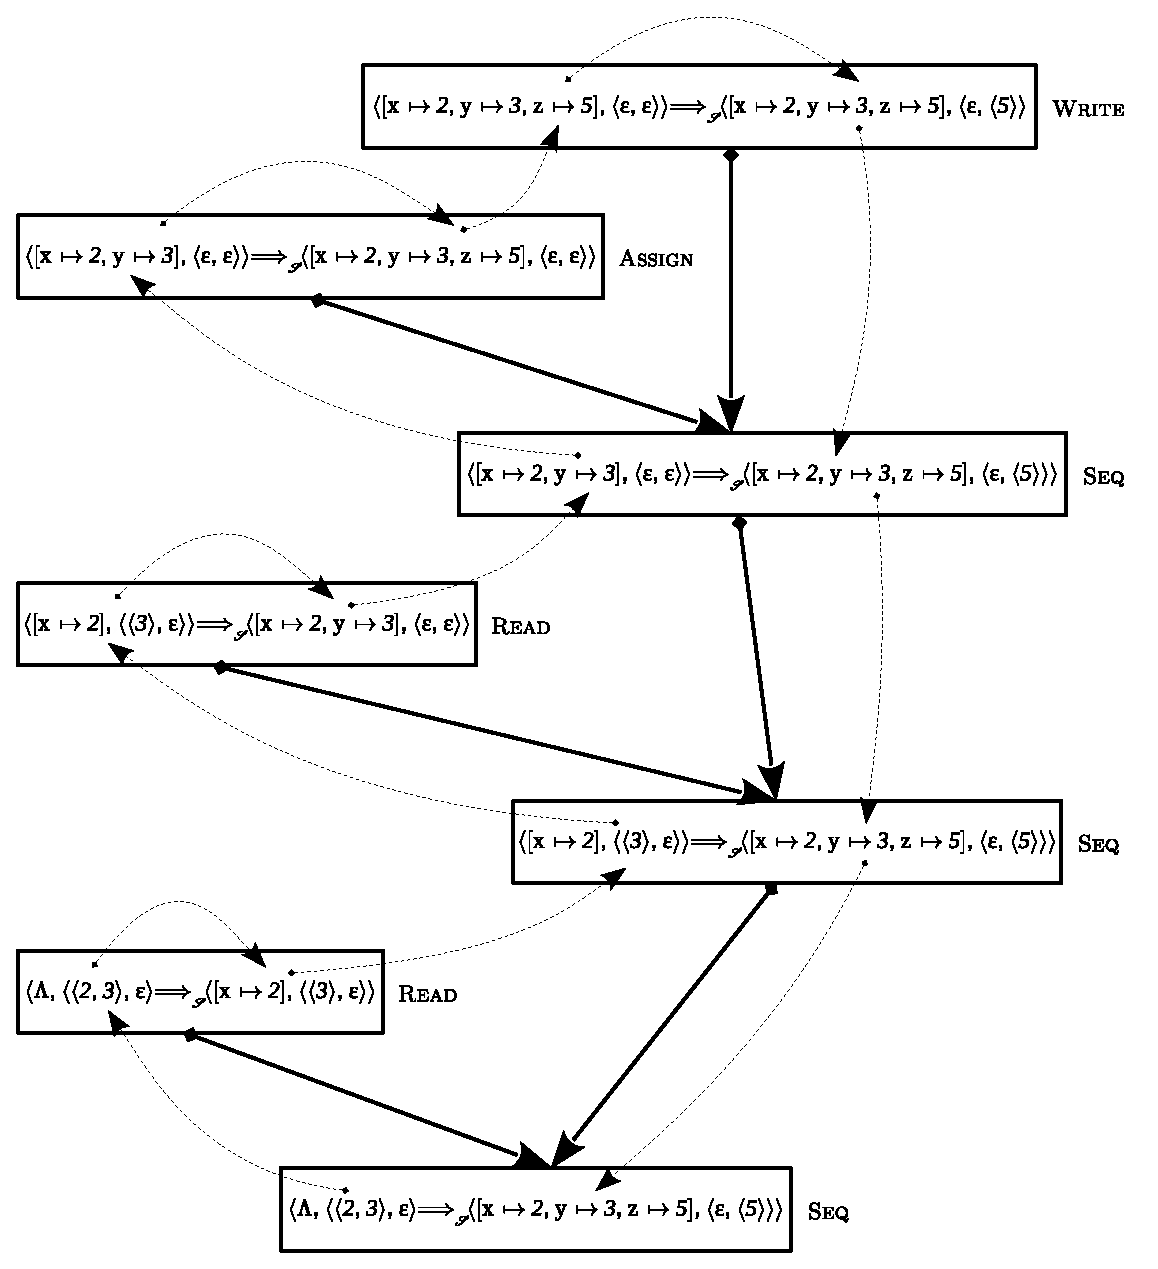
\includegraphics[scale=0.8]{images/03-01.eps}
  \caption{Derivation tree example}
  \label{derivation-tree}
\end{figure}

We can see that big-step operational semantics allows us to perform program evaluation for concrete input: we just form an initial configuration for this input and then
systematically apply rules of the semantics until (and if) we come to the result of the evaluation. The application of an axiom completes in one
step (we can immediately evaluate the result configuration); the application of the rule for sequential composition amounts to splitting the composite
statement into two, moving one floor up in the semantics's rule, and repeat. In the process a certain structure, called \emph{derivation tree}, is
maintained implicitly. The nodes of a derivation tree are \emph{instances} of the semantics' rules, the edges connect premises with conclusions. The derivation
tree for the example we just considered is depictured in Fig.~\ref{derivation-tree} (the program's statements are omitted due to space considerations). Additionally
to the derivation tree itself a configuration calculation flow is shown explicitly by dashed arrows. We can see, that for axioms these arrows come directly from
left- to right-hand part of the rules, while the rule for composition threads configurations from right-hard part of one rule to the left-hand part of another.

\FloatBarrier

Besides evaluation big-step operational semantics can also be used to \emph{prove} the properties of the programs. For example, we can prove, that for
arbitrary $n,\, m\in\mathbb{N}$ 

\[
\sembr{\llang{read (x); read (y); z := x + y; write (z)}}^\ph_\mathscr{S}\,\inbr{n,\,m}=n+m
\]

Indeed, we just need to repeat the construction of the derivation tree as we did in the evluation case, but this time instead of concrete numbers use
their abstract denotations $n$ and $m$; all steps could be performed as before until we arrive at the assignment rule. This time we would need to prove
an additional lemma

\[
\sembr{\llang{x + y}}^\ph_\mathscr{E}\,[\llang{x}\mapsto n,\,\llang{y}\mapsto m]=n+m
\]

which, of course, can be easily done by unfolding corresponding rule for $\sembr{\bullet}^\ph_\mathscr{E}$.

And, besides proving the properties of \emph{concrete programs}, big-step operational semantics can be used to prove the properties
of the semantics of the \emph{language} as whole. We consider some examples in the next section.

\subsection{Properties of the Semantics}

Now we formulate some simple properties of the semantics for straight-line programs; as the language is rather simple, these
properties and their proofs might look obvious. We nevertheless do this as a set of warming-up exersices to demonstrate
relevant techniques before dealing with more advanced languages with less trivial properties.

\subsubsection{Associativity of Composition}

First we consider rather an expected property of sequential composition to be \emph{associative}.

\begin{lemma}[Associativity of composition] For arbitrary $s_1,\,s_2,\,s_3$ and arbitrary $c_1,\,c_2$

\[
\trans{c_1}{\llang{$s_1$; ($s_2$; $\,s_3$)}}{c_2}\xLeftrightarrow{\phantom{XXX}}{}\trans{c_1}{\llang{($s_1$; $\,s_2$); $\,s_3$}}{c_2}
\]


In other words, the grouping of statements inside compositions is not essential, only their order.
\end{lemma}

\begin{proof}
Proving this claim amounts to
proving it in both directions; we only do it from left to right since the opposite can be done similarly. So, we assume

\[
\trans{c_1}{\llang{$s_1$; ($s_2$; $\,s_3$)}}{c_2}\eqno{(\star)}
\]

From this it is immedialety follows that

\[
\trule{\trans{c_1}{s_1}{c^\prime}\quad\trans{c^\prime}{\llang{$s_2$; $\,s_3$}}{c_2}}
      {\trans{c_1}{\llang{$s_1$; ($s_2$; $\,s_3$)}}{c_2}}
\]

because there is no way to complete the derivation tree for $(\star)$ other than by applying the rules of the semantics (this time, $\rulename{Seq}$).
Similarly, we can apply the same rule for the second premise, which gives us

\[
\trule{\trans{c_1}{s_1}{c^\prime}\qquad\trule{\trans{c^\prime}{s_2}{c^{\prime\prime}}\quad\trans{c^{\prime\prime}}{s_3}{c_2}}{\trans{c^\prime}{\llang{$s_2$; $\,s_3$}}{c_2}}}
      {\trans{c_1}{\llang{$s_1$; ($s_2$; $\,s_3$)}}{c_2}}
\]

Thus, we may conclude, that

\[
\begin{array}{c}
  \trans{c_1}{s_1}{c^\prime}\\
  \trans{c^\prime}{s_2}{c^{\prime\prime}}\\
  \trans{c^{\prime\prime}}{s_3}{c_2}
\end{array}
\]

for some configurations $c^\prime$ and $c^{\prime\prime}$. Now we turn our attention to the following evaluation relation:

\[
\trans{c_1}{\llang{($s_1$; $\,s_2$); $\,s_3$}}{\fbox{?}}
\]

We have to prove that $\fbox{?}=c_2$; again, applying rule $\rulename{Seq}$ twice we arrive at (a partial) derivation tree

\[
\trule{\trule{\trans{c_1}{s_1}{\fbox{???}}\quad\trans{\fbox{???}}{s_2}{\fbox{??}}}
             {\trans{c_1}{\llang{$s_1$; $\,s_2$}}{\fbox{??}}}\qquad\trans{\fbox{??}}{s_3}{\fbox{?}}}
      {\trans{c_1}{\llang{($s_1$; $\,s_2$); $\,s_3$}}{\fbox{?}}}
\]

By the determinism of the semantics we can conclude that $\fbox{???}=c^\prime$, from which (again, by determinism) immediately follows that
$\fbox{??}=c^{\prime\prime}$ and, finally, that $\fbox{?}=c_2$.
\end{proof}

Note, we did not use anything besides the rule $\rulename{Seq}$, thus
the associativity of composition does not depend on other rules and will hold as long as the rule $\rulename{Seq}$
is kept in its current form.

From what we've just proven it is immediately follows that for arbitrary $s_1,\,s_2,\,s_3$ 

\[
\sembr{\llang{$s_1$; ($s_2$; $\,s_3$)}}^\ph_\mathscr{S}=\sembr{\llang{($s_1$; $\,s_2$); $\,s_3$}}^\ph_\mathscr{S}
\]

In other words, regrouping the components of composition is an equivalent transformation.

\subsubsection{Finite Read and Write}

The next property we are going to establish is that every statement can read only a finite number of input
stream elements; this number depends only on the statement itself, and for all initial configurations with an input stream
shorter than that number the evaluation never comes to a final configuration. Formally, we prove the following lemma:

\begin{lemma}[Finite read] For any statement $s$ there is a natural number $n$ such that for every configuration $c=\inbr{\sigma,\,\inbr{i,\,o}}$

\begin{enumerate}
\item if $|i|<n$ then there is no configuration $c^\prime$ such that $\trans{c}{s}{c^\prime}$;
\item if $|i|\ge n$ and there is some configuration $c^\prime=\inbr{\sigma^\prime,\,\inbr{i^\prime,\,o^\prime}}$ such that $\trans{c}{s}{c^\prime}$, then
  $|i^\prime|=|i|-n$.
\end{enumerate}

\end{lemma}

\begin{proof}   
The proof goes by structural induction. For the base case we need to consider four simple statements and four corresponding semantics rules.
By inspecting the rules $\rulename{Skip}$, $\rulename{Assign}$, and $\rulename{Write}$ we can conclude that neither of them touches input stream. Thus,
if an evaluation according to these rules succesfully completes, then input streams of initial and final configurations are equal. This means that for these
three statements $n=0$.

On the contrary, the rule $\rulename{Read}$ takes one element from input stream and puts it into a state. In the final configuration input stream will be one
element shorter, and this configuration can not be constructed if the initial one had empty input stream. Thus, in this case $n=1$.

To complete the proof, we need to perform an induction step by inspecting the rule $\rulename{Seq}$. Let us have a statement $s_1\llang{;}s_2$; by
induction hypothesis we may conclude, that there are numbers $n_1$ and $n_2$ such the claim is true for $s_1$ and $s_2$, respectively. Let first
assume, that for some configuration $c=\inbr{\sigma,\,\inbr{i,\,o}}$ there is another one $c^\prime=\inbr{\sigma^\prime,\,\inbr{i^\prime,\,o^\prime}}$ such that

\[
\trans{c}{s_1\llang{;}s_2}{c^\prime}
\]

By unfolding the rule $\rulename{Seq}$ we have


\[
\trule{\trans{c}{s_1}{\inbr{\sigma^{\prime\prime},\,\inbr{i^{\prime\prime},\,o^{\prime\prime}}}}\quad\trans{\inbr{\sigma^{\prime\prime},\,\inbr{i^{\prime\prime},\,o^{\prime\prime}}}}{s_2}{c^\prime}}
      {\trans{c}{s_1\llang{;}s_2}{c^\prime}}
\]

From induction hypothesis for $s_1$ we know, that $|i^{\prime\prime}|=|i|-n_1$; from induction hypothesis for $s_2$ we know, that $|i^\prime|=|i^{\prime\prime}|-n_2$; thus, overall
$|i^\prime|=|i|-n_1-n_2$, or $|i^\prime|=|i|-(n_1+n_2)$ and $n=n_1+n_2$.

Let us now assume that $|i|<n_1+n_2$. If $|i|<n_1$, then, by the induction hypothesis for $s_1$, there is no configuration $c^{\prime\prime}$ such that

\[
\trans{\inbr{\sigma,\,\inbr{i,\,o}}}{s_1}{c^{\prime\prime}}
\]

If $n_1\le|i|<n_1+n_2$ and there is a configuration $c^{\prime\prime}=\inbr{\sigma^{\prime\prime},\,\inbr{i^{\prime\prime},\,o^{\prime\prime}}}$ such that

\[
\trans{\inbr{\sigma,\,\inbr{i,\,o}}}{s_1}{c^{\prime\prime}}
\]

then $|i^{\prime\prime}|<n_2$ by induction hypothesis for $s_1$; by induction hypothesis for $s_2$ there is no configuration $c^\prime$ such that

\[
\trans{c^{\prime\prime}}{s_2}{c^\prime}
\]

which completes the proof.
\end{proof}

A similar property can be established for output streams.

\begin{lemma}[Finite write] Let $s$ be a statement. Then there is a natural number $n$ such that for each
pairs of configurations $c=\inbr{\sigma,\,\inbr{i,\,o}}$ and $c^\prime=\inbr{\sigma^\prime,\,\inbr{i^\prime,\,o^\prime}}$ if

\[
\trans{c}{s}{c^\prime}
\]

then $|o^\prime|=|o|+n$.
\end{lemma}

\begin{proof}
  Like in the previous lemma, the principle of structural induction gives us the blueprint for the proof.
  In the base case, we consider four simple statements and corresponding semantics rules. For all cases, except for
  $\rulename{Write}$, the output stream is left untouched, thus $n=0$. For $\rulename{Write}$, if the statement
  managed to succeed, the output stream in the final configuration is one element longer, than in the initial
  one, thus $n=1$.

  In the induction step case, we have a statement $s_1\llang{;}s_2$ and we assume that lemma holds for $s_1$ and $s_2$; this
  gives us the numbers $n_1$ and $n_2$. Next we assume that

  \[
  \trans{c}{s_1\llang{;}s_2}{c^\prime}
  \]

  and unfold the rule $\rulename{Seq}$:

  \[
  \trule{\trans{c}{s_1}{\inbr{\sigma^{\prime\prime},\,\inbr{i^{\prime\prime},\,o^{\prime\prime}}}}\quad\trans{\inbr{\sigma^{\prime\prime},\,\inbr{i^{\prime\prime},\,o^{\prime\prime}}}}{s_2}{c^\prime}}
        {\trans{c}{s_1\llang{;}s_2}{c^\prime}}
  \]


  By induction hypothesis for $s_1$ we know that $|o^{\prime\prime}|=|o|+n_1$; by induction hypothesis for $s_2$~--- that $|o^\prime|=|o^{\prime\prime}|+n_2$. Thus, $|o^\prime|=|o|+(n_1+n_2)$, from
  which we conclude $n=n_1+n_2$.
\end{proof}

We can see the similarity between these two proofs; to tell the truth this is the case for all claims that can be proven by structural induction. Thus, almost every time
when we encounter such a claim we will skip the proof.

From these two lemmas we can derive the following corollaries:

\begin{enumerate}
\item For arbitrary $s\in\mathscr{S}$,$\,i,\,i^\prime\in\mathbb{Z}^*$ if both $\sembr{s}^\ph_\mathscr{S}\,i$ and $\sembr{s}^\ph_\mathscr{S}\,i^\prime$ defined, then
  \[
  |\sembr{s}^\ph_\mathscr{S}\,i|=|\sembr{s}^\ph_\mathscr{S}\,i^\prime|
  \]

  In other words, the length of the result depends only on the statement, not input data.

\item
  Let $\sembr{s}^\ph_\mathscr{S}\,i$ is defined for some $s\in\mathscr{S}$ and $i\in\mathbb{Z}^*$. Then for arbitrary $i^\prime\in\mathbb{Z}^*$

  \[
   \sembr{s}^\ph_\mathscr{S}\,ii^\prime=\sembr{s}^\ph_\mathscr{S}\,i
   \]

   In other words, if a program has returned some result for some input, it will also return the same result
   if we arbitrarily extend this input. The proof uses the determinism property of the semantics.
\end{enumerate}

\subsubsection{Variable Renaming}

The last example of a semantic property we are going to consider is \emph{equivalence up to variable renaming}.

By observing the semantics of expressions and statements we may notice that to some extent all variables
are indistinguishable: no rule requires any \emph{specific} variable to be used, any variable can be potentially used
anywhere. Thus, if we, for example, have an assignment

\begin{lstlisting}[mathescape=true]
   a := $E$
\end{lstlisting}

we can rename ``\lstinline|a|'' in, say, ``\lstinline|b|'', and nothing changes as long as we simultaneously
rename all following occurrencies of ``\lstinline|a|'' to ``\lstinline|b|'' as well. We have, however, to be
careful to avoid  \emph{coalescing} different variables into one; for example, if ``\lstinline|b|'' already
used in the same program, the result of renaming may or may not be correct depending on the properties
of this concrete program. Thus, we should only consider \emph{one-to-one} variable renamings.

More formally, we call a function

\[
\theta : \mathscr{X}\to\mathscr{X}
\]

a \emph{renaming} iff the following two conditions hold:

\begin{enumerate}
\item $\theta$ is total (defined for each $x\in\mathscr{X}$);
\item for each $y\in\mathscr{X}$ there is a unique $x\in\mathscr{X}$ such that $\theta\,(x)=y$.
\end{enumerate}

This is in fact a mathematical definition of a \emph{bijective} mapping from $\mathscr{X}$ to $\mathscr{X}$.
It is immediately follows from the definition that the inverse mapping $\theta^{-1}$ exists, which is
also a bijection. Moreover, both compositions $\theta\theta^{-1}$ and $\theta^{-1}\theta$ are identity
functions.

We now define what is a result of application of a renaming $\theta$ to an expression $e$ (notation: $e\,\theta$):

\[
\begin{array}{rclcl}
  x\,\theta&=&\theta\,(x)&,&x\in\mathscr{X}\\
  n\,\theta&=&n&,&n\in\mathbb{N}\\
  (l\oplus r)\,\theta&=&(l\,\theta)\oplus(r\,\theta)&
\end{array}
\]

In a nutshell, $e\,\theta$ is an expression in which all variables are substituted to their images according to $\theta$.
Similarly, we can extend the application of renaming to statements:

\[
\begin{array}{rcl}
  \llang{skip}\,\theta&=&\llang{skip}\\
  (x\llang{:=}e)\,\theta&=&(\theta\,(x))\llang{:=}(e\,\theta)\\
  (\llang{read ($x$)})\,\theta&=&\llang{read ($\theta\,(x)$)}\\
  (\llang{write ($e$)})\,\theta&=&\llang{write ($e\,\theta$)}\\
  (s_1\llang{;}s_2)\,\theta&=&(s_1\,\theta)\llang{;}(s_2\;\theta)
\end{array}
\]

\begin{lemma}
  Let $s$ be a statement and $\theta$ be a renaming. Then

  \[
  s\equiv s\,\theta
  \]
\end{lemma}
\begin{proof}
  First, we recollect that

  \[
  s\equiv s\,\theta
  \]

  means precisely

  \[
  \sembr{s}^\ph_\mathscr{S}=\sembr{s\,\theta}^\ph_\mathscr{S}
  \]

  Since $\sembr{\bullet}^\ph_\mathscr{S}$ is defined in terms of evaluation relation ``$\transrel$'' we need to prove
  a similar claim for ``$\transrel$''. This claim on the first glance may look like the follows: for all $c,\,c^\prime\in\mathscr{C}$

  \[
  \trans{c}{s}{c^\prime}\xLeftrightarrow{\phantom{XXX}}{}\trans{c}{s\,\theta}{c^\prime}
  \]

  Alas, this does not hold in general case: let us have a statement $\llang{write ($x$)}$ and let
  $\theta\,(x)=y$. Then for a configuration $c=\inbr{[x\mapsto 3],\,\inbr{i,\,o}}$ there is no $c^\prime$
  such that

  \[
  \trans{c}{\llang{write ($y$)}}{c^\prime}
  \]

  since $y$ is undefined in $[x\mapsto 3]$. The problem here is that renamed statements only behave similarly to the original ones
  in \emph{renamed} states.

  The fixed claim looks like the follows: let $c=\inbr{\sigma,\,w}$ and $c^\prime=\inbr{\sigma^\prime,\,w^\prime}$ then

  \[
  \trans{c}{s}{c^\prime}\xLeftrightarrow{\phantom{XXX}}{}\trans{\inbr{\sigma\circ\theta^{-1},\,w}}{s\,\theta}{\inbr{\sigma^\prime\circ\theta^{-1},\,w^\prime}}\eqno{(\clubsuit)}
  \]

  Informally speaking here we ``repair'' states for renamed statements by first applying the \emph{inverse} renaming $\theta^{-1}$ which exists by bijectivity of $\theta$. To
  prove this we need additional claim.

  \begin{claim}[$\spadesuit$]
    Let $e$ be an expression, $\sigma$ be a state, and $n$ be an integer number. Then

    \[
    \sembr{e}^\ph_\mathscr{E}\,\sigma=n \xLeftrightarrow{\phantom{XXX}}{}\sembr{e\,\theta}^\ph_\mathscr{E}\,(\sigma\circ\theta^{-1})=n
    \]
  \end{claim}
  \begin{proof}
    One may expect that the proof has to be performed in two directions. However, by the bijectivity of $\theta$

    \[
    \begin{array}{rcl}
      \theta&=&(\theta^{-1})^{-1}\\
      (e\,\theta)\,\theta^{-1}&=&e\\
      \sigma&=&(\sigma\circ\theta^{-1})\circ\theta
    \end{array}
    \]

    Thus, if we prove the claim from left to right, then (by arbitrariness of $e$, $\sigma$, and $\theta$) we can
    assume

    \[
    \begin{array}{rcl}
      e&=&e\,\theta\\
      \sigma&=&\sigma\circ\theta^{-1}
    \end{array}
    \]

    and the right-to-left direction will follow from left-to-right immediately.
    
    The proof proceeds by structural induction.

    The base case is a constant or a variable. Since the semantics of constants does not depend on a state the
    claim for constant case follows vacuously. If $e$ is a variable $x$, then:

    \[
    \begin{array}{rcl}
      \sembr{x\,\theta}^\ph_\mathscr{E}\,(\sigma\circ\theta^{-1})&=&\mbox{(by the definition of $\sembr{\bullet}^\ph_\mathscr{E}$)}\\
      (\sigma\circ\theta^{-1})\,(x\,\theta)&=&\mbox{(by the definition of renaming application)}\\
      (\sigma\circ\theta^{-1})\,(\theta\,(x))&=&\mbox{(by the definition of function composition)}\\
      ((\sigma\circ\theta^{-1})\circ\theta)\,(x)&=&\mbox{(by the associativity of function composition)}\\
      (\sigma\circ(\theta^{-1}\circ\theta))\,(x)&=&\mbox{(by the definition of function inversion)}\\
      \sigma\,(x)&=&\mbox{(by the condition of the claim)}\\
      n&&
    \end{array}
    \]

    The induction step assumes that the claim holds for some expressions $l$ and $r$; we need to prove that it also holds for
    $l\oplus r$:

    \[
    \begin{array}{rcl}
      \sembr{(l\oplus r)\,\theta}\,(\sigma\circ\theta^{-1})&=&\mbox{(by the definition of renaming application)}\\
      \sembr{(l\,\theta)\oplus(r\,\theta)}\,(\sigma\circ\theta^{-1})&=&\mbox{(by the definition of $\sembr{\bullet}^\ph_\mathscr{E}$)}\\
      \sembr{l\,\theta}\,(\sigma\circ\theta^{-1})\otimes\sembr{r\,\theta}\,(\sigma\circ\theta^{-1})&=&\mbox{(by inductive hypotheses)}\\
      \sembr{l}\,\sigma\otimes\sembr{r}\,\sigma&=&\mbox{(by the condition of the claim)}\\
      n&&      
    \end{array}
    \]

    This completes the proof.
  \end{proof}

  The proof of $(\clubsuit)$ goes by structural induction as well. Similarly to the claim $(\spadesuit)$ we only need to prove it in
  one direction (let it be left-to-right).

  In the base case we have to consider four types of simple statements:

  \begin{enumerate}
  \item As $\llang{skip}$ does not change a configuration the lemma holds vacuously.
  \item Let us have an assignment $x\llang{:=}e$. First, by the definition of renaming application

    \[
    (x\llang{:=}e)\,\theta=(\theta\,(x))\llang{:=}(e\,\theta)
    \]

    Then, by the definition of ``$\transrel$'':
    
    \[
    \trans{\inbr{\sigma\circ\theta^{-1},\,w}}{(\theta\,(x))\llang{:=}(e\,\theta)}{\inbr{(\sigma\circ\theta^{-1})[\theta\,(x)\gets\sembr{e\,\theta}^\ph_\mathscr{E}\,(\sigma\circ\theta^{-1})],\,w}}
    \]

    By $(\spadesuit)$ we know that

    \[
    \sembr{e\,\theta}^\ph_\mathscr{E}\,(\sigma\circ\theta^{-1})=\sembr{e}^\ph_\mathscr{E}\,\sigma
    \]

    By the definition of substitution in a state

    \[
    (\sigma\circ\theta^{-1})[\theta\,(x)\gets\sembr{e}^\ph_\mathscr{E}\,\sigma]\,y=\left\{\begin{array}{rcl}
                                                                                         \sembr{e}^\ph_\mathscr{E}\,\sigma&,&y=\theta\,(x)\\
                                                                                         (\sigma\circ\theta^{-1})\,y&,&y\ne\theta\,(x)
                                                                                       \end{array}\right.
    \]

    By the properties of functional inversion and composition and, again, using the definition of substitution in a state we have

    \[
    \left\{\begin{array}{rcl}
                                                                                         \sembr{e}^\ph_\mathscr{E}\,\sigma&,&y=\theta\,(x)\\
                                                                                         (\sigma\circ\theta^{-1})\,y&,&y\ne\theta\,(x)
                                                                                       \end{array}\right.=
   \left\{\begin{array}{rcl}
   \sembr{e}^\ph_\mathscr{E}\,\sigma&,&\theta^{-1}\,(y)=x\\
   (\sigma\,(\theta^{-1}\,(y))&,&\theta^{-1}\,(y)\ne x
    \end{array}\right.=(\sigma[x\gets\sembr{e}^\ph_\mathscr{E}])\,(\theta^{-1}\,(y))
    \]

    Thus, $\sigma^\prime=\sigma[x\gets\sembr{e}^\ph_\mathscr{E}]\circ\theta^{-1}$ which completes the proof for the assignment case.
    
  \item Two remaining cases can be proven similarly using the observation that worlds are invariant under renaming.
    
  \end{enumerate}
  
  Finally, to prove the induction step we assume that $(\clubsuit)$ holds for statements $s_1$ and $s_2$ and we need
  to prove

  \[
  \trans{\inbr{\sigma\circ\theta^{-1},\,w}}{s_1\llang{;}s_2}{\inbr{\sigma^\prime\circ\theta^{-1},\,w^\prime}}
  \]

  From the condition of the lemma we know

  \[
  \trule{\trans{\inbr{\sigma,\,w}}{s_1}{\inbr{\sigma^{\prime\prime},\,w^{\prime\prime}}}\quad\trans{\inbr{\sigma^{\prime\prime},\,w^{\prime\prime}}}{s_2}{\inbr{\sigma^\prime,\,w^\prime}}}
        {\trans{\inbr{\sigma,\,w}}{s_1\llang{;}s_2}{\inbr{\sigma^\prime,\,w^\prime}}}
  \]

  for some $\sigma^{\prime\prime}$ and $w^{\prime\prime}$. Applying the induction hypotheses to the premises and then applying rule $\rulename{Seq}$ we acquire the following
  derivation

  \[
  \trule{\trans{\inbr{\sigma\circ\theta^{-1},\,w}}{s_1}{\inbr{\sigma^{\prime\prime}\circ\theta^{-1},\,w^{\prime\prime}}}\quad\trans{\inbr{\sigma^{\prime\prime}\circ\theta^{-1},\,w^{\prime\prime}}}{s_2}{\inbr{\sigma^\prime\circ\theta^{-1},\,w^\prime}}}
        {\trans{\inbr{\sigma\circ\theta^{-1},\,w}}{s_1\llang{;}s_2}{\inbr{\sigma^\prime\circ\theta^{-1},\,w^\prime}}}
  \]

  which proves the induction step.

  Now, assume

  \[
  \trans{\inbr{\Lambda,\,\inbr{i,\,\epsilon}}}{s}{\inbr{\sigma,\,w}}
  \]

  By $(\clubsuit)$ we have

  \[
  \trans{\inbr{\Lambda\circ\theta^{-1},\,\inbr{i,\,\epsilon}}}{s\,\theta}{\inbr{\sigma\circ\theta^{-1},\,w}}
  \]

  But $\Lambda\circ\theta^{-1}=\Lambda$, which completes the proof since now we have 

  \[
  \sembr{s}^\ph_\mathscr{E}\,i=\sembr{s\,\theta}^\ph_\mathscr{E}\,i
  \]

  for arbitrary $i$ by the definition of $\sembr{\bullet}^\ph_\mathscr{E}$.
  
\end{proof}

\begin{comment}
First, we define the set of all \emph{free variables} $\fv{}$ in expression or statement:

\[
\begin{array}{rclcl}
  \fv{x} &=& \{x\}&,& x\in\mathscr{X}\\
  \fv{z} &=&\emptyset &,&z\in\mathbb{N}\\
  \fv{l\oplus r} &=& \fv{l}\cup\fv{r}&&
\end{array}
\]

\[
\begin{array}{rcl}
  \fv{\llang{skip}}&=&\emptyset\\
  \fv{x\,\llang{:=}\,e}&=&\{x\}\cup\fv{e}\\
  \fv{\llang{read ($x$)}}&=&\{x\}\\
  \fv{\llang{write ($e$)}}&=&\fv{e}\\
  \fv{s_1\llang{;}s_2}&=&\fv{s_1}\cup\fv{s_2}xs  
\end{array}
\]
\end{comment}


\end{document}
